% !TeX spellcheck = en_GB
%%%%%%%%%%%%%%%%%%%%%%%%%%%%%%%%%%%%%%%%%%
%                                        %
%    Engineer thesis LaTeX template      % 
%                                        %
%%%%%%%%%%%%%%%%%%%%%%%%%%%%%%%%%%%%%%%%%%



\documentclass[a4paper,twoside,12pt]{book}
\usepackage[utf8]{inputenc}                                      
\usepackage[T1]{fontenc}  
\usepackage{amsmath,amsfonts,amssymb,amsthm}
\usepackage[polish,british]{babel} 
\usepackage{indentfirst}
\usepackage{lmodern}
\usepackage{graphicx} 
\usepackage{hyperref}
\usepackage{booktabs}
\usepackage{tikz}
\usepackage{pgfplots}
\usepackage{mathtools}
\usepackage{geometry}
\usepackage[page]{appendix} 

\usepackage{setspace}
\usepackage{array}
\onehalfspacing


\frenchspacing

\usepackage{listings}
\lstset{
	language={},
	basicstyle=\ttfamily,
	keywordstyle=\lst@ifdisplaystyle\color{blue}\fi,
	commentstyle=\color{gray}
}

%%%%%%%%%

 

%%%%%%%%%%%% FANCY HEADERS %%%%%%%%%%%%%%%

\usepackage{fancyhdr}
\pagestyle{fancy}
\fancyhf{}
\fancyhead[LO]{\nouppercase{\it\rightmark}}
\fancyhead[RE]{\nouppercase{\it\leftmark}}
\fancyhead[LE,RO]{\it\thepage}


\fancypagestyle{onlyPageNumbers}{%
   \fancyhf{} 
   \fancyhead[LE,RO]{\it\thepage}
}

\fancypagestyle{PageNumbersChapterTitles}{%
   \fancyhf{} 
   \fancyhead[LO]{\nouppercase{\it\rightmark}}
   \fancyhead[RE]{\nouppercase{\it\leftmark}}
   \fancyhead[LE,RO]{\it\thepage}
}


%%%%%%%%%%%%%%%%%%%%%%%%%%%
% listings 
\usepackage{listings}
\lstset{%
language=C++,%
commentstyle=\textit,%
identifierstyle=\textsf,%
keywordstyle=\sffamily\bfseries, %\texttt, %
%captionpos=b,%
tabsize=3,%
frame=lines,%
numbers=left,%
numberstyle=\tiny,%
numbersep=5pt,%
breaklines=true,%
morekeywords={descriptor_gaussian,descriptor,partition,fcm_possibilistic,dataset,my_exception,exception,std,vector},%
escapeinside={@*}{*@},%
%texcl=true, % wylacza tryb verbatim w komentarzach jednolinijkowych
}
%%%%%%%%%%%%%%%%%%%%%%%%%%%%%%%%%%%%

%%%% TODO LIST GENERATOR %%%%%%%%%

\usepackage{color}
\definecolor{brickred}      {cmyk}{0   , 0.89, 0.94, 0.28}

\makeatletter \newcommand \kslistofremarks{\section*{Remarks} \@starttoc{rks}}
  \newcommand\l@uwagas[2]
    {\par\noindent \textbf{#2:} %\parbox{10cm}
{#1}\par} \makeatother


\newcommand{\remark}[1]{%
{%\marginpar{\textdbend}
{\color{brickred}{[#1]}}}%
\addcontentsline{rks}{uwagas}{\protect{#1}}%
}

%%%%%%%%%%%%%% END OF TODO LIST GENERATOR %%%%%%%%%%% 

% some issues...

\newcounter{PagesWithoutNumbers}

\newcommand{\hcancel}[1]{%
    \tikz[baseline=(tocancel.base)]{
        \node[inner sep=0pt,outer sep=0pt] (tocancel) {#1};
        \draw[red] (tocancel.south west) -- (tocancel.north east);
    }%
}%

\newcommand{\MonthName}{%
  \ifcase\the\month
  \or January% 1
  \or February% 2
  \or March% 3
  \or April% 4
  \or May% 5
  \or June% 6
  \or July% 7
  \or August% 8
  \or September% 9
  \or October% 10
  \or November% 11
  \or December% 12
  \fi}


%%%%%%%%%%%%%%%%%%%%%%%%%%%%%%%%%%%%%%%%%%%%%%
% Helvetica font macros for the title page:
\newcommand{\headerfont}{\fontfamily{phv}\fontsize{18}{18}\bfseries\scshape\selectfont}
\newcommand{\titlefont}{\fontfamily{phv}\fontsize{18}{18}\selectfont}
\newcommand{\otherfont}{\fontfamily{phv}\fontsize{14}{14}\selectfont}

%%%%%%%%%%%%%%%%%%%%%%%%%%%%%%%%%%%%%%%%%%%%%%
%%%%%%%%%%%%%%%%%%%%%%%%%%%%%%%%%%%%%%%%%%%%%%
%%%%%%%%%%%%%%%%%%%%%%%%%%%%%%%%%%%%%%%%%%%%%%
%%%%%%%%%%%%%%%%%%%%%%%%%%%%%%%%%%%%%%%%%%%%%%
%%%%%%%%%%%%%%%%%%%%%%%%%%%%%%%%%%%%%%%%%%%%%%
%%%%%%%%%%%%%%%%%%%%%%%%%%%%%%%%%%%%%%%%%%%%%%
%%%%%%%%%%%%%%%%%%%%%%%%%%%%%%%%%%%%%%%%%%%%%%
\newcommand\tabularhead[2]{
\begin{table}%[h!]
  \caption{<<#1>> #2}
  \begin{tabular}{|p{0.4\linewidth}|p{0.55\linewidth}|}
    \hline
    \textbf{Action} & \textbf{#1} \\
    \hline}

  \newcommand\addrow[2]{#1 &#2\\ \hline}

  \newcommand\addmulrow[2]{ \begin{minipage}[t][][t]{2.5cm}#1\end{minipage}% 
     &\begin{minipage}[t][][t]{8cm}
      \begin{enumerate} #2   \end{enumerate}
      \end{minipage}\\ }

  \newenvironment{usecase}{\tabularhead}
{\hline\end{tabular}\end{table}}

\newcommand{\Author}{Adam Gajewski}
\newcommand{\Supervisor}{Krzysztof Dobosz, PhD}
%\newcommand{\Consultant}{Name Surname, PhD}
\newcommand{\Title}{Development of accessible mobile sudoku}
\newcommand{\Polsl}{Silesian University of Technology}
\newcommand{\Faculty}{Faculty of Automatic Control, Electronics and Computer Science}


\usepackage{float}

\begin{document} 
	
%%%%%%%%%%%%%%%%%%  Title page %%%%%%%%%%%%%%%%%%% 
\pagestyle{empty}
{
	\newgeometry{top=2.5cm,%
	             bottom=2.5cm,%
	             left=3cm,
	             right=2.5cm}
	\sffamily
	\rule{0cm}{0cm}
	
	\begin{center}
	
\includegraphics[width=29mm]{polsl}
	\end{center} 
	\vspace{1cm}
	\begin{center}
	\headerfont \Polsl
	\end{center}
	\begin{center}
	\headerfont \Faculty
	\end{center}
	\vfill
	\begin{center}
	\titlefont Engineer  thesis
	\end{center}
	\vfill
	
	\begin{center}
	\otherfont \Title\par
	\end{center}
	
	\vfill
	
	\vfill
	 
	\noindent\vbox
	{
		\hbox{\otherfont author: \Author}
		\vspace{12pt}
		\hbox{\otherfont supervisor: \Supervisor}
		\vspace{12pt}
		%\hbox{\otherfont consultant: \Consultant}
	}
	\vfill 
 
   \begin{center}
   \otherfont Gliwice,  \MonthName\ \the\year
   \end{center}	
	\restoregeometry
}
  

\cleardoublepage
 

\rmfamily
\normalfont


%%%%%%%%%%%% statements required by law and Dean's office %%%%%%%%%%
\cleardoublepage

\begin{flushright}
załącznik nr 2 do zarz. nr 97/08/09 
\end{flushright}

\vfill  

\begin{center}
\Large\bfseries Oświadczenie
\end{center}

\vfill

\underline{Wyrażam  zgodę} / Nie wyrażam zgody*  na  udostępnienie  mojej  \underline{pracy  dyplomowej} / rozprawy doktorskiej*.

\vfill

Gliwice, dnia {\selectlanguage{polish}\today}

\vfill

\rule{0.5\textwidth}{0cm}\dotfill 

\rule{0.5\textwidth}{0cm}
\begin{minipage}{0.45\textwidth}
{\begin{center}(podpis)\end{center}}
\end{minipage} 

\vfill

\rule{0.5\textwidth}{0cm}\dotfill 

\rule{0.5\textwidth}{0cm}
\begin{minipage}{0.45\textwidth}
{\begin{center}\rule{0mm}{5mm}(poświadczenie wiarygodności podpisu przez Dziekanat)\end{center}}
\end{minipage}


\vfill

* podkreślić właściwe

 


%%%%%%%%%%%%%%%%%%%%%  
\cleardoublepage

\rule{1cm}{0cm}

\vfill  

\begin{center}
\Large\bfseries Oświadczenie promotora
\end{center}

\vfill

Oświadczam, że praca „\Title” spełnia wymagania formalne pracy dyplomowej inżynierskiej.

\vfill



\vfill

Gliwice, dnia {\selectlanguage{polish}\today}

\rule{0.5\textwidth}{0cm}\dotfill 

\rule{0.5\textwidth}{0cm}
\begin{minipage}{0.45\textwidth}
{\begin{center}(podpis promotora)\end{center}}
\end{minipage} 

\vfill
 
 

\cleardoublepage


%%%%%%%%%%%%%%%%%% Table of contents %%%%%%%%%%%%%%%%%%%%%%
\pagenumbering{Roman}
\pagestyle{onlyPageNumbers}
\tableofcontents

%%%%%%%%%%%%%%%%%%%%%%%%%%%%%%%%%%%%%%%%%%%%%%%%%%%%%
\setcounter{PagesWithoutNumbers}{\value{page}}
\mainmatter
\pagestyle{PageNumbersChapterTitles}

%%%%%%%%%%%%%% body of the thesis %%%%%%%%%%%%%%%%%


\chapter{Introduction}

\iffalse
\begin{itemize}
\item introduction into the problem domain
\item settling of the problem in the domain
\item objective of the thesis 
\item scope of the thesis
\item short description of chapters
%\item clear description of contribution of the thesis's author – in case of more authors table with enumeration of contribution of authors
\end{itemize}
\fi

%\clearpage

\section{Introduction into the problem domain}

\par Sudoku is a logic-based, combinatorial number-placement puzzle\cite{bib:sudoku}. The objective is to fill a 9x9 grid with digits so that each column, each row, and each of the nine 3x3 subgrids that compose the grid (later on called "cells" in this thesis) contains all of the digits from 1 to 9. Under the name "Mini Sudoku", a 6x6 variant with 3x2 regions appears in the many newspapers. The object is the same as that of standard Sudoku, but the puzzle only uses the numbers 1 through 6.
\par
Accessibility is a feature that lets blind people to use smartphones. Even if an application was not designed for blind people, they mostly still can use it thanks to screen readers like TalkBack (an accessibility service for Android) reading out loud the content of app to the user. It is a small help compere to many problems related to being blind, but we can increase this help, by creating applications that are more accessible friendly.
\par
Due to the fact that in order to know what is the content of something that is currently displayed on the screen, a specific part of the screen must be tapped, the application should not use the same event as the chose action. In TalkBack this event is overwritten by double tap, so after first tap a button (for example) TalkBack tells the user what was just tapped. After a double tap the application calls the same action as if this element was tapped once with TalkBack turned off. Using TalkBack changes this and many other behaviors of applications, which can make many applications unable to work properly. To change this back to how the application worked originally without TalkBack, the application have to be designed either disable some of TalkBack features for parts of itself, or overwrite its reactions to touch events.
\par
The easiest accessible thing to implement is some text to read. To any other elements should be provided appropriate labels. Thanks to that most of visual features can be forgotten and the user can proceed to use the app. One of problems of this solution is time necessary for the audio to be played. Because of that application requiring faster response are a lot harder to be accessible, so there are not many accessible games on smartphones.

\section{Settling of the problem in the domain}
\par
Making an accessible game we can take one of two approaches: Either we make the UI simple and decrease number of elements on screen to minimum, or we take the risk of making something more complicated. In the first case we just have to think of an idea that does not require from the user to chose from many options or to react very fast. It leaves us with really lot of options: Quizzes, text RPG's, crosswords, and so on. Simple design does not make a game boring, everything depends on the execution. In the second case we must put trust in the user and make a bit more complicated UI with more elements. When the user will get used to the game this difference in difficulty should decrease, but the time for learning how to play will be usually longer, than in the first case.

\section{Objective of the thesis}

\par The main objective is to create a working accessible Sudoku game that can be solved both by a blind person and someone fully sighted. The solution should be compatible with support software used by visually disabled users.
\par Communication with any external systems is not planned..

\iffalse
\titleformat{\chapter}[display]
  {\normalfont\sffamily\huge\bfseries}
  {\chaptertitlename\ \thechapter}{5pt}
  {\begin{flushleft}
  \normalfont\normalsize\textit{Here is the place where the description of each chapter goes. \vspace{0.25cm}}
  \end{flushleft}
  \Huge}
\fi

\section{Short description of chapters}

\par The thesis is constructed of following chapters:

\begin{itemize}
\item Introduction - Short description of accessible solutions domain, and what the thesis is going to be about.
\item Problem analysis - Problems in the game development accessible for people with visual disabilities, and description of similar solutions of mobile Sudoku applications.
\item Requirements and tools - Requirements concerning behavior of the application, its main features, and compatibility with system and tools.
\item External specification - Usage and requirements of the application.
\item Internal specification - Description of the program and its structure. Analysis of the code and components.
\item Verification and validation - Testing process and results of the performed tests.
\item Conclusions - Conclusions and final results of the project.
\end{itemize}

\chapter{Problem analysis}


%\iffalse
%\begin{itemize}
%\item  problem analysis
%\item state of the art, problem statement
%\item  literature research (all sources in the thesis have to be referenced \cite{bib:internet})
%\item description of existing solutions (also scientific ones, if the problem is scientifically researched), algorithms,  location of the thesis in the scientific domain
%\end{itemize}

%\clearpage
%\fi

\section {User characteristics}

\par There are a many different visual conditions that could limit a person trying to play a game. The primary conditions encountered in gaming are limitations in vision are:\cite{bib:internet}

\begin{itemize}
\item Blindness - usually defined as “the loss of vision, not correctable with lenses”. People who are completely blind cannot play games that rely on visual cues to prompt a player. They must rely on sounds or special hardware such as force feedback to indicate when they need to act.
\item Low Vision:
\begin{itemize}
\item Low vision is related to blindness. A person with low vision can detect light, perhaps see some motion, but is very limited as to what they can see.
A more detailed definition of low vision is “a visual acuity of 20/70 or worse in the better eye using a best-corrected spectacle correction, or visual fields of twenty degrees or fewer.
\item However, a more functional definition is that low vision comprises any vision loss that adversely affects the performance of daily activities.” A related term is “legally blind”. “Legal blindness is defined as visual acuity of 20/200 or worse in the better eye with correction, or visual fields of twenty degrees or fewer in the better eye“.
\item In either of these cases, users could play games provided there was some degree of magnification of the screen. Users could respond to visual and sound cues, but their ability to see a wide area of the game may be restricted by the magnification of the screen.
\end{itemize}
\item Color Blindness:
\begin{itemize}
\item Color blindness is an inability to detect certain colors. It ranges from total color blindness, where the person perceives the world as shades of gray, to more common types where a person does not perceive the differences between red and green or yellow and blue correctly.
\item This condition is more common among men than women. Studies have shown that from 5 to 8\% of all men and about 0.5\% of women have some degree of color blindness.
\item The effects of color blindness are more pronounced under certain game color schemes. An example from the past was the Firaxis game “Sid Meier’s Alpha Centauri”. The primary color scheme was mostly red and green, which caused problems for some players. This was quickly addressed through the release of a patch, which provided alternate art for the game. Figure \ref{fig:centauri} Example of bad combination of colors. Between 5\% and 8\% of men have some kind of colorblindness, so using color to differentiate friendly units from enemy units could make the game unplayable for millions of people\cite{bib:colorblind}.\
	\end{itemize}
\end{itemize}

\begin{figure}
\centering
  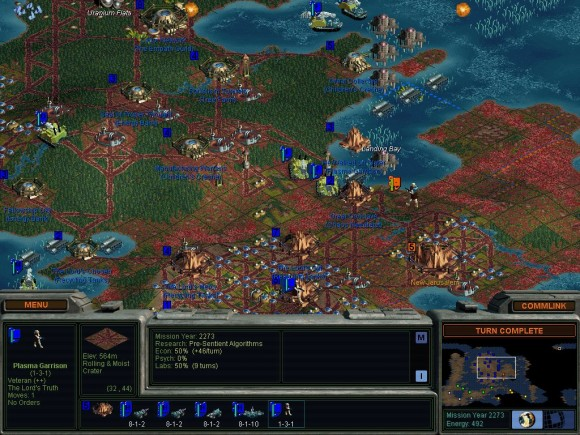
\includegraphics[width=\linewidth/2]{centauri.jpg}
  \caption{Sid Meier’s Alpha Centauri - Example of bad combination of colors}
  \label{fig:centauri}
\end{figure}

%\par Included informations from: accessible.games\cite{bib:internet}.

\par The most popular advices in making accessible games for people with visual conditions are
\begin{itemize}
	\item Keep your color palette limited to 2 or 3 colors.
	\item Avoid using bad color combinations.
	\item Carefully select any contrasting colors and shades.
	\item Don’t only rely on color to convey a message.
	\item Use simple font against a plain background.
	\item Use appropriate font size\cite{bib:dzone}.
\end{itemize}

\par And for the game to be really accessible, it cannot exclude deaf people. Users with hearing impairments include deaf people, as well as people with partial hearing or hearing loss in one or multiple ears. There are a number of other hearing disorders but these are the main ones we can combat with accessible design. That is why using both visual and audio elements is very important for accessibility.

\par
The smartphone accessible games have been available for a few years, and the conventional ones were more common for even longer. Puzzles like Rubik cube with braille alphabet on it can be found easily, and there exists a similar solution for the Sudoku puzzle, with numbers represented by small blocks with braille number on it, that can be putted into the puzzle. That solution can not be used in an electronic device not having any form of system showing braille alphabet. There exists a solution on the descktop computer using keyboard and audio reading content of the sudoku, but agin nowadays smartphones usully do not have keyboaeds. 

\section {Existing mobile sudoku applications}

\par
Durring working on this thesis there heve not been found any accessible sudoku applications. Figures \ref{fig:Sudoku app1} and \ref{fig:Sudoku app2} are presenting classical Sudoku applications.
\iffalse
\begin{figure}[H]
\centering
  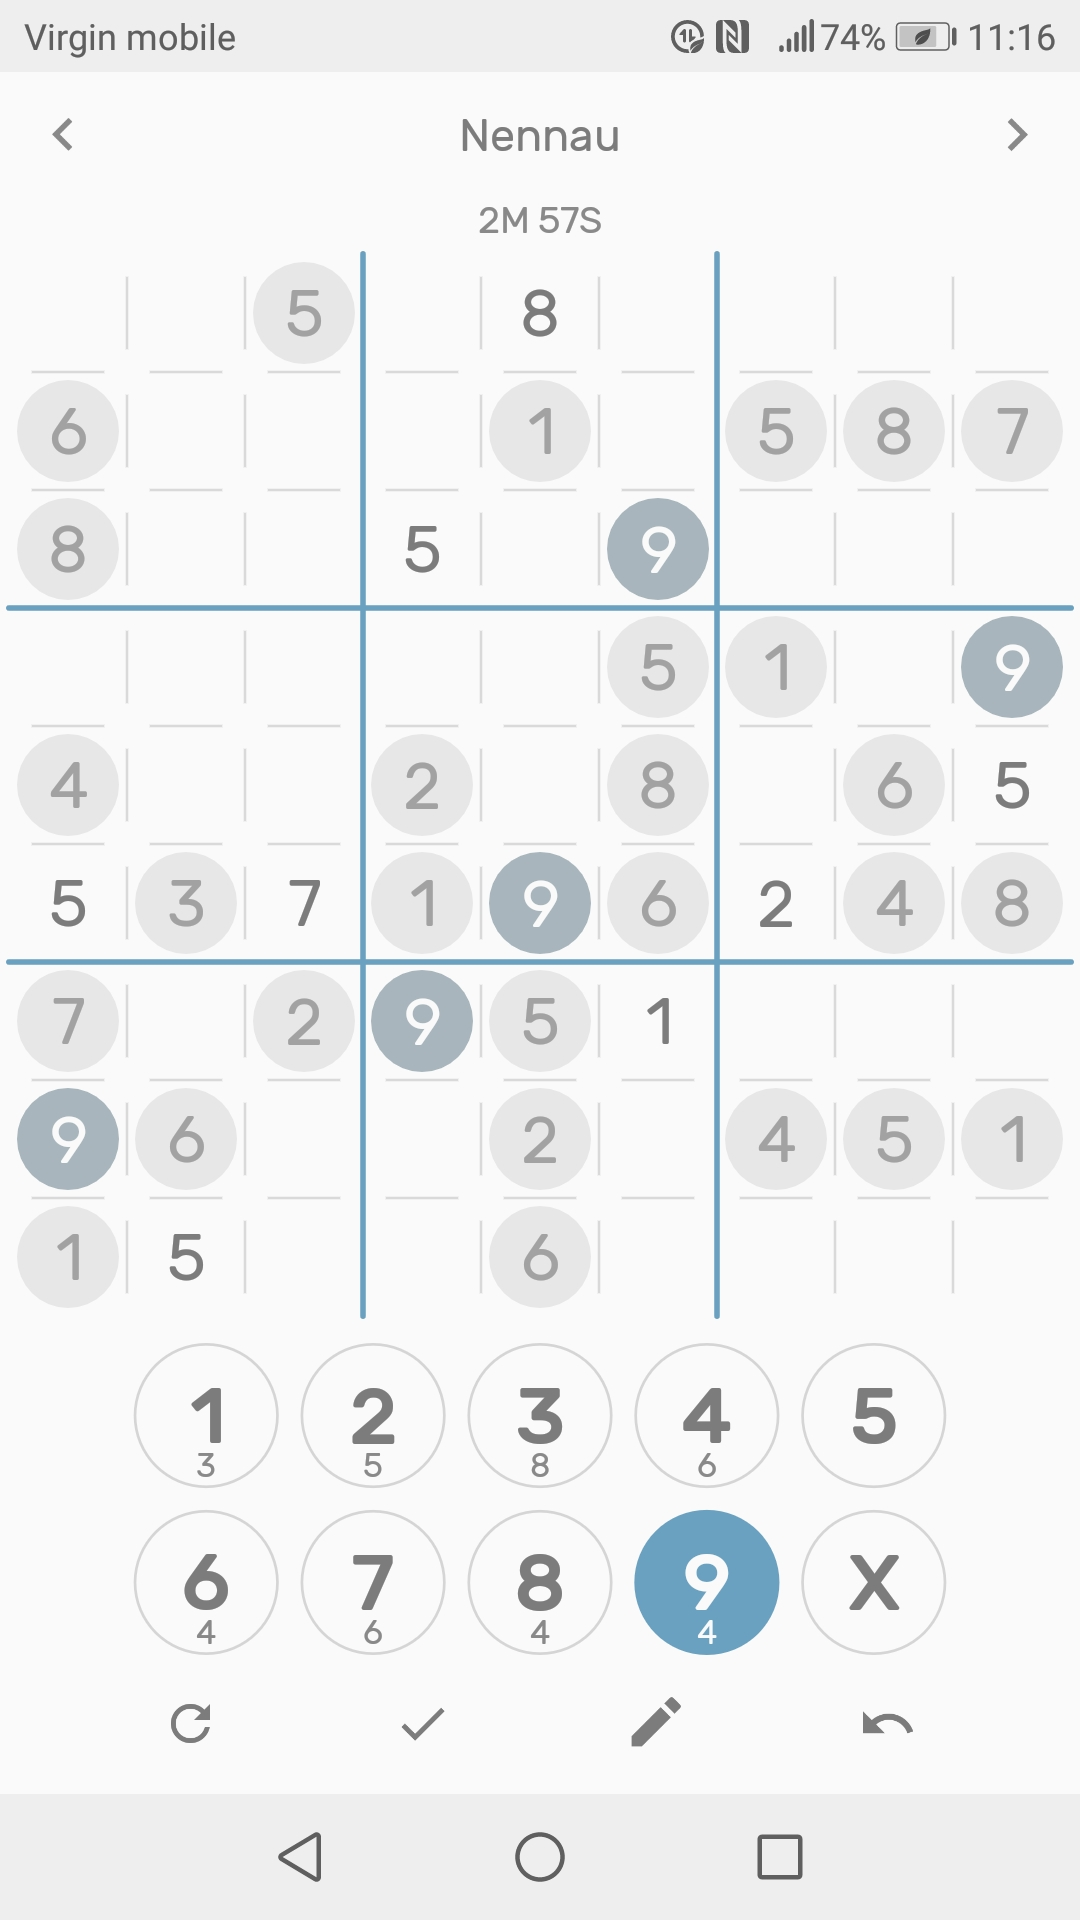
\includegraphics[width=\linewidth/4]{sudoku.jpg}
  \caption{Sudoku.}
  \label{fig:Sudoku1}
%\end{centering}
\end{figure}
\fi

%Figure \ref{fig:Sudoku1} normal sudoku application.

\begin{figure}[H]
\centering
\begin{minipage}{.5\textwidth}
  \centering
  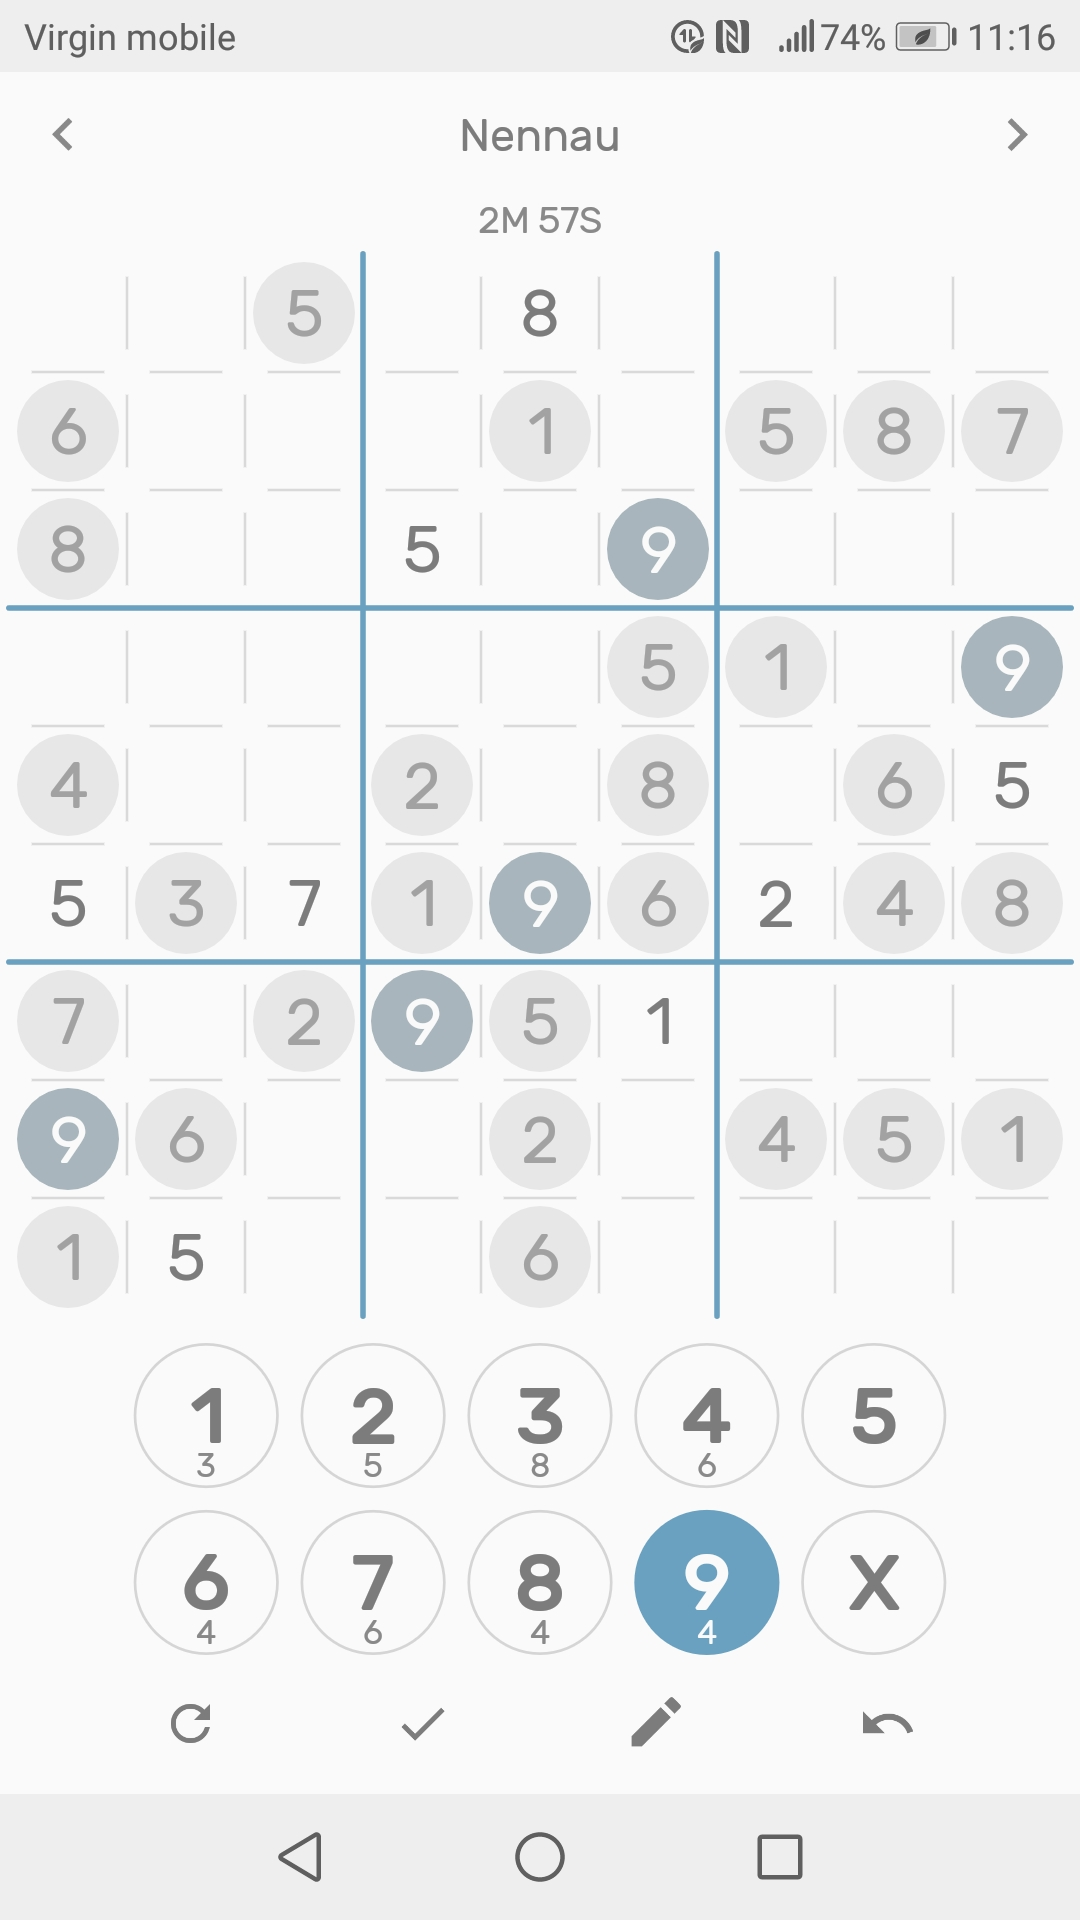
\includegraphics[width=.8\linewidth]{sudoku.jpg}
  \caption{Sudoku app1}
  \label{fig:Sudoku app1}
\end{minipage}%
\begin{minipage}{.5\textwidth}
  \centering
  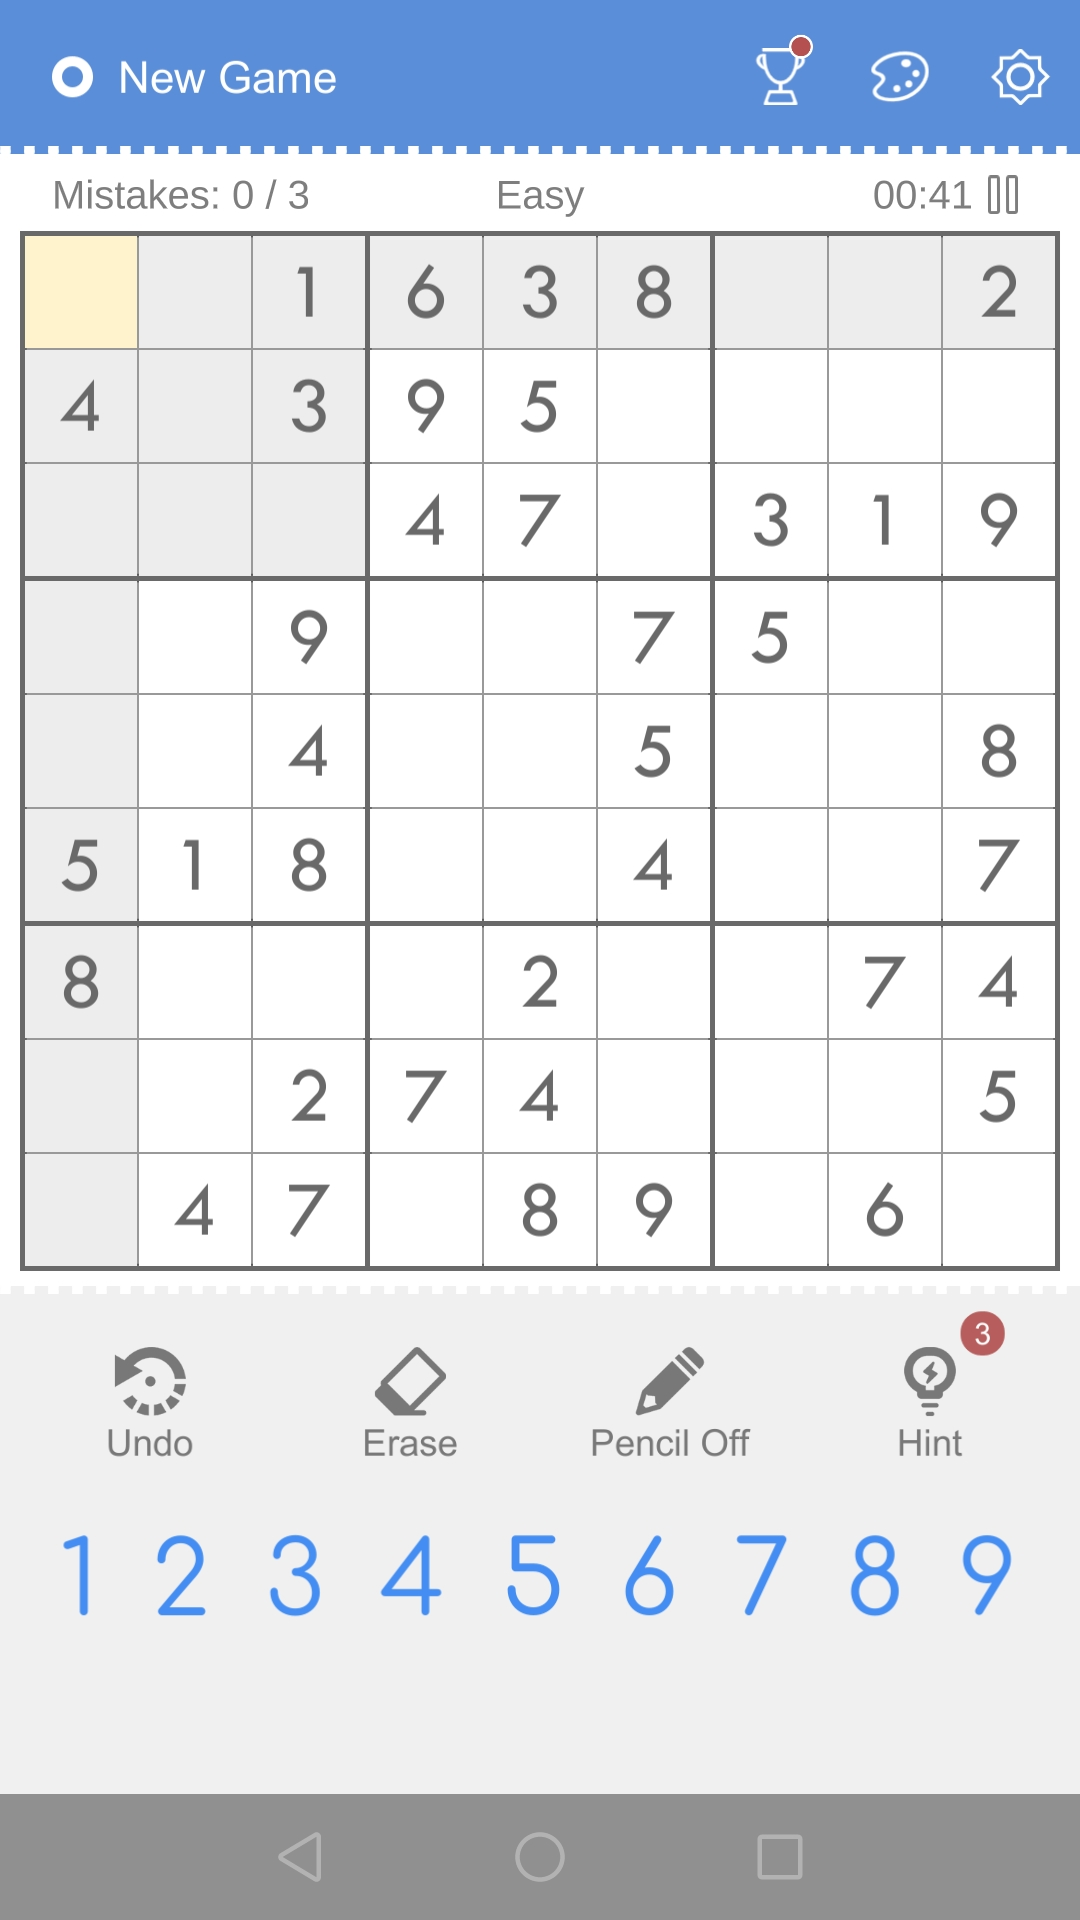
\includegraphics[width=.8\linewidth]{sudoku2.jpg}
  \caption{Sudoku app2}
  \label{fig:Sudoku app2}
\end{minipage}
\end{figure}

\begin{figure}[H]
  \centering
  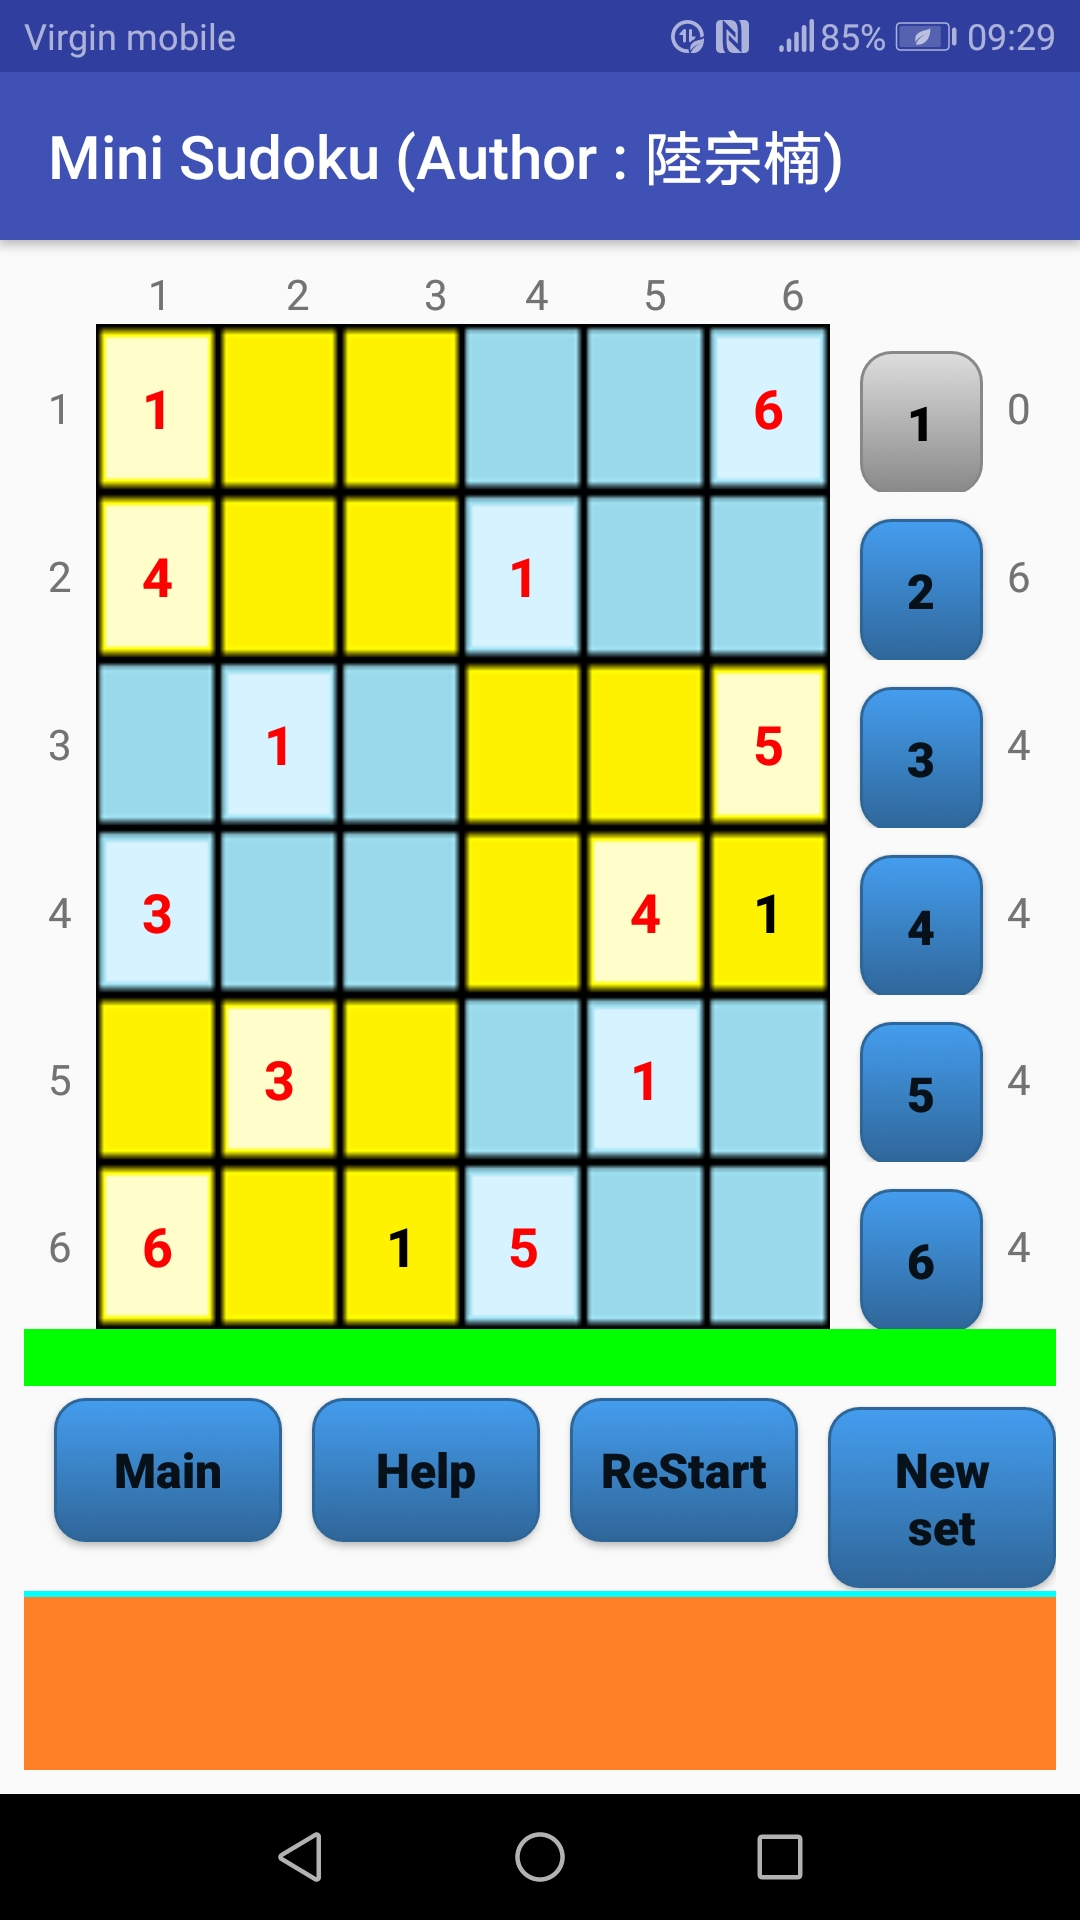
\includegraphics[width=.4\linewidth]{sudoku3.jpg}
  \caption{Small Sudoku app}
  \label{fig:Small Sudoku app}
\end{figure}

\par Most of the tested applications could be used with TalkBack turned on, because all the game functions became disabled, and even if those functions would work as they were without TalkBack, a person with high visual disability could not use it, because TalkBack could not read the content of the application, and there was not any interface implemented instead to tell the user the content of the Sudoku.
\par The only Sudoku application found during work on this thesis was a simplified version of sudoku shown on figure \ref{fig:Small Sudoku app}. Despite the fact it is not an application designed for visually disabled people it still can be used by them.

\section {Existing mobile accessible games}

\par TapBeats is open-source project created for the Winter 2011 Accessibility Capstone at the University of Washington. It has simple user interface based on views with instructions and views having four buttons filling in the screen (figure \ref{fig:Tap beats instruction} and figure \ref{fig:Tap beats game}). This way those elements are easier to find for a blind user. Its text to speech system is using the TalkBack from the device to communicate information to the user. The behavior of this application does not visibly change after turning the TalkBack on, and the usage stays the same.

\begin{figure}[!hb]
\centering
\begin{minipage}{.5\textwidth}
  \centering
  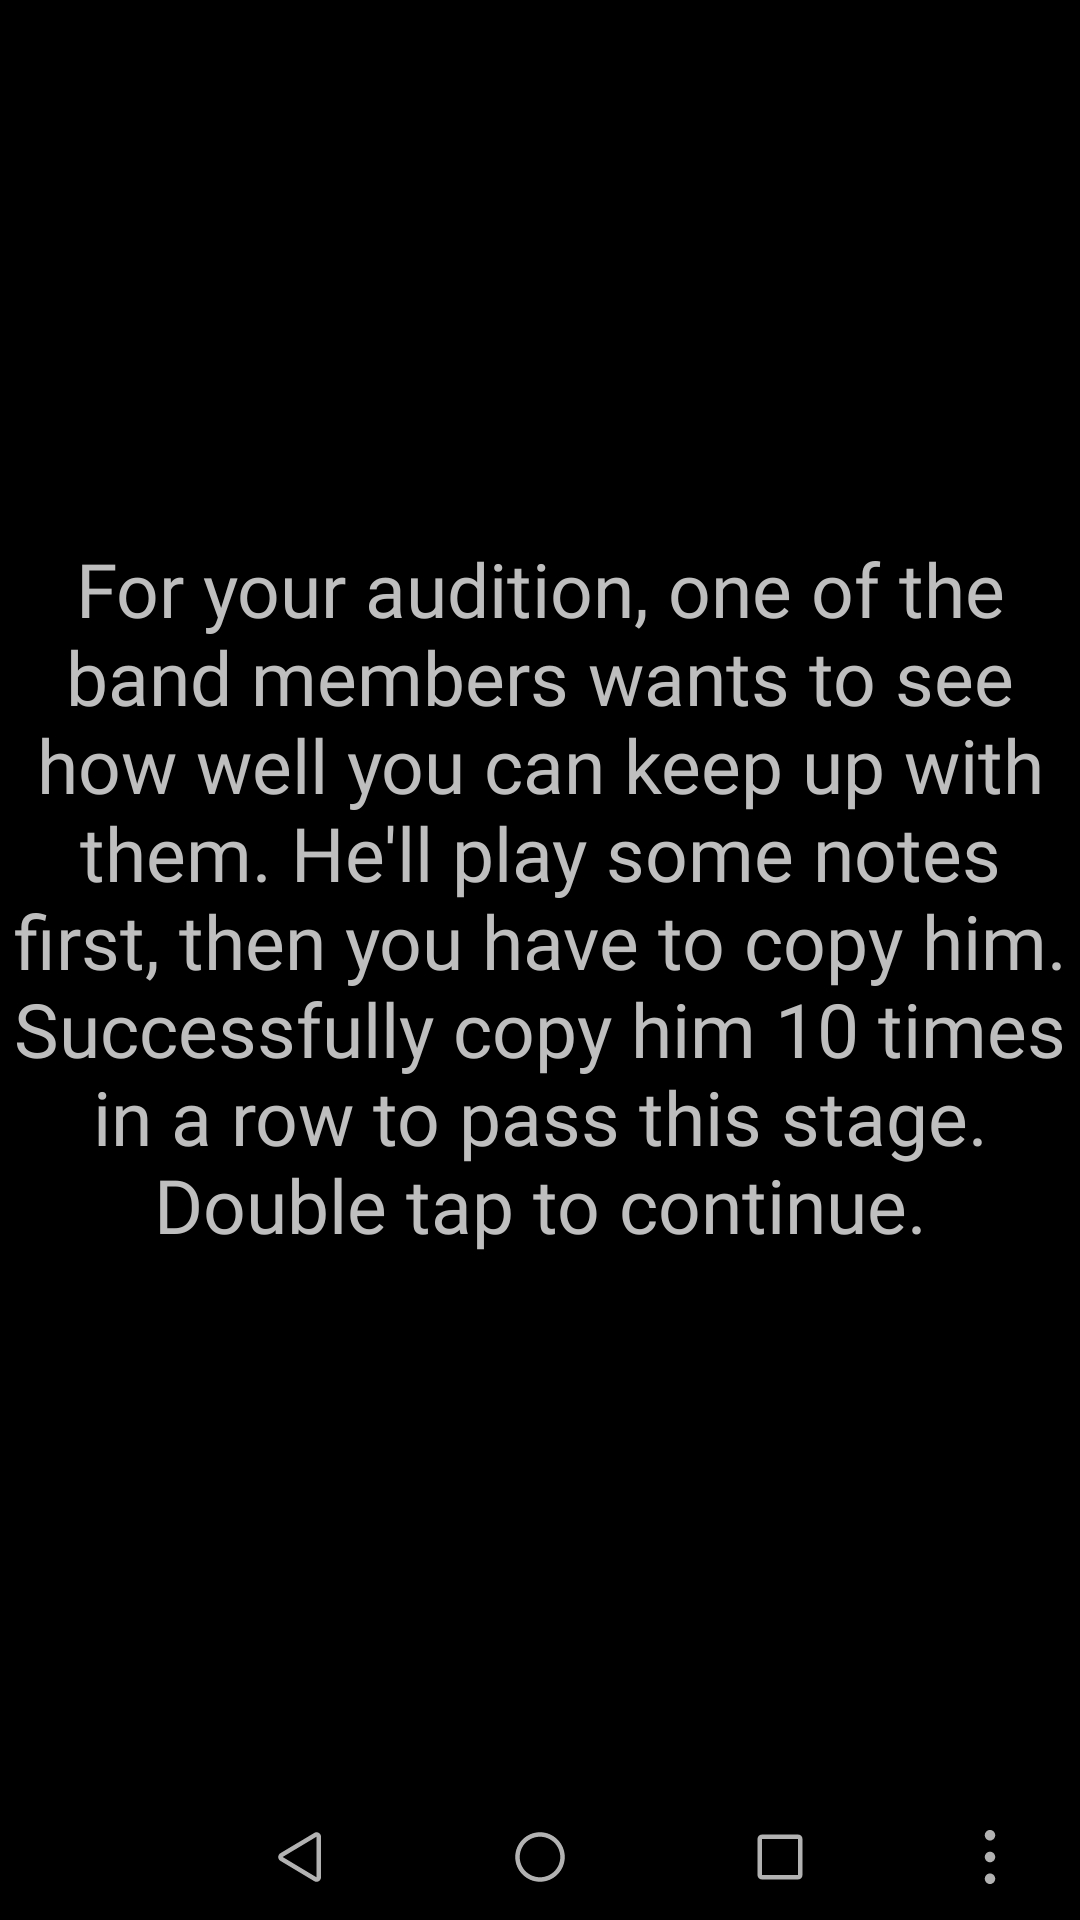
\includegraphics[width=.8\linewidth]{tapbit instruction.jpg}
  \caption{Tap beats instruction}
  \label{fig:Tap beats instruction}
\end{minipage}%
\begin{minipage}{.5\textwidth}
  \centering
  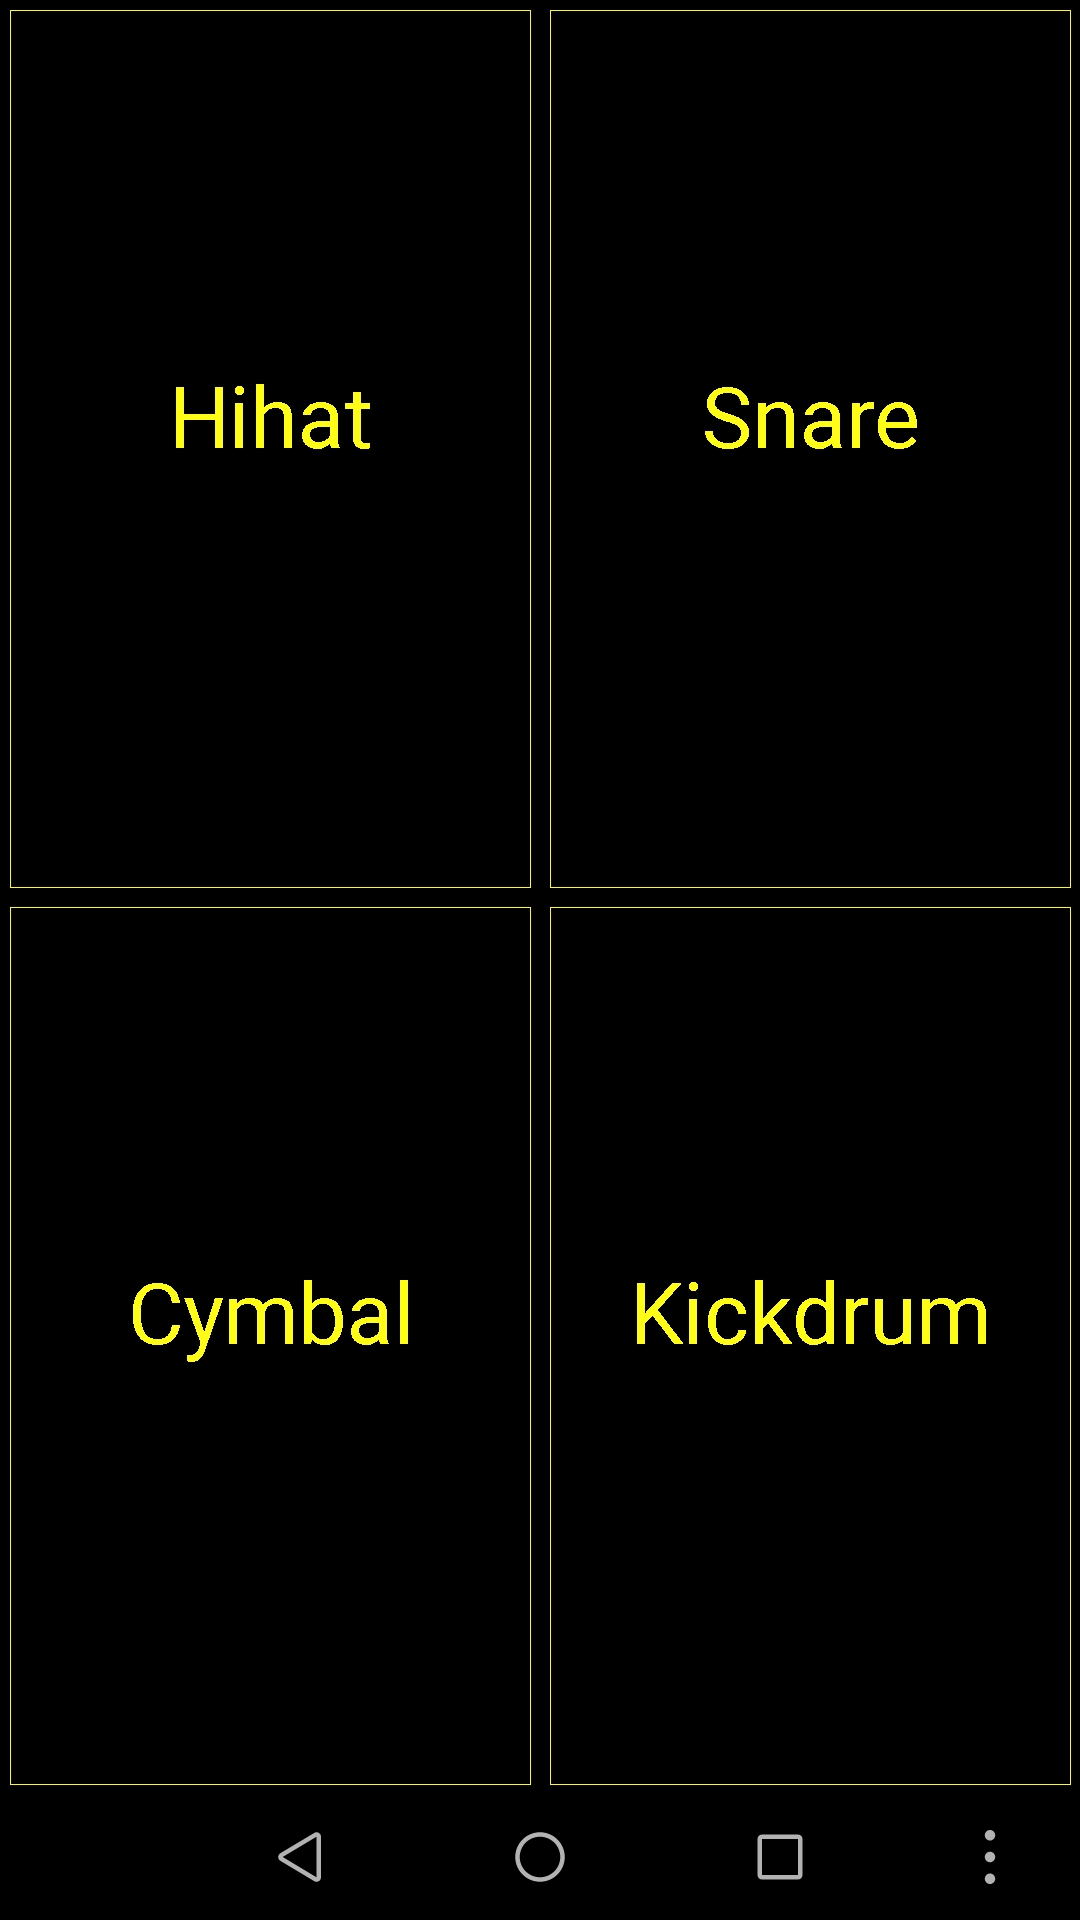
\includegraphics[width=.8\linewidth]{tapbit.jpg}
  \caption{Tap beats game}
  \label{fig:Tap beats game}
\end{minipage}
\end{figure}

\par Audio Game Hub is mobile application with games based on sounds. It can be used by a blind player, as the user interface and menu are based on TalkBack behavior. Usage of the application is simple as it is explained in the tutorial step by step to the user, and the elements on the screen are placed in order that is easy to imagine and only some elements is shown at a time (figure ref{audio hub menu}), as more menu items can be accessed by swiping up and down. The games themselves are using sounds to represent the state of the game. The game shown on the figure \ref{fig:audio hub blocks} is called Blocks. Its objective is to place together 3 elements (blocks) with the same color (sound). The blocks are falling from the above and the player have limited time to decide in which column it should be placed. Even thou that not seeing the game makes it for a blind user harder to play, it is still possible.
\par Unfortunately the application is not compatible with the TalkBack, and cannot be used with it. Its only way of dealing with this problem is asking the user to turn the TalkBack off.

\begin{figure}[H]
\centering
\begin{minipage}{.5\textwidth}
  \centering
  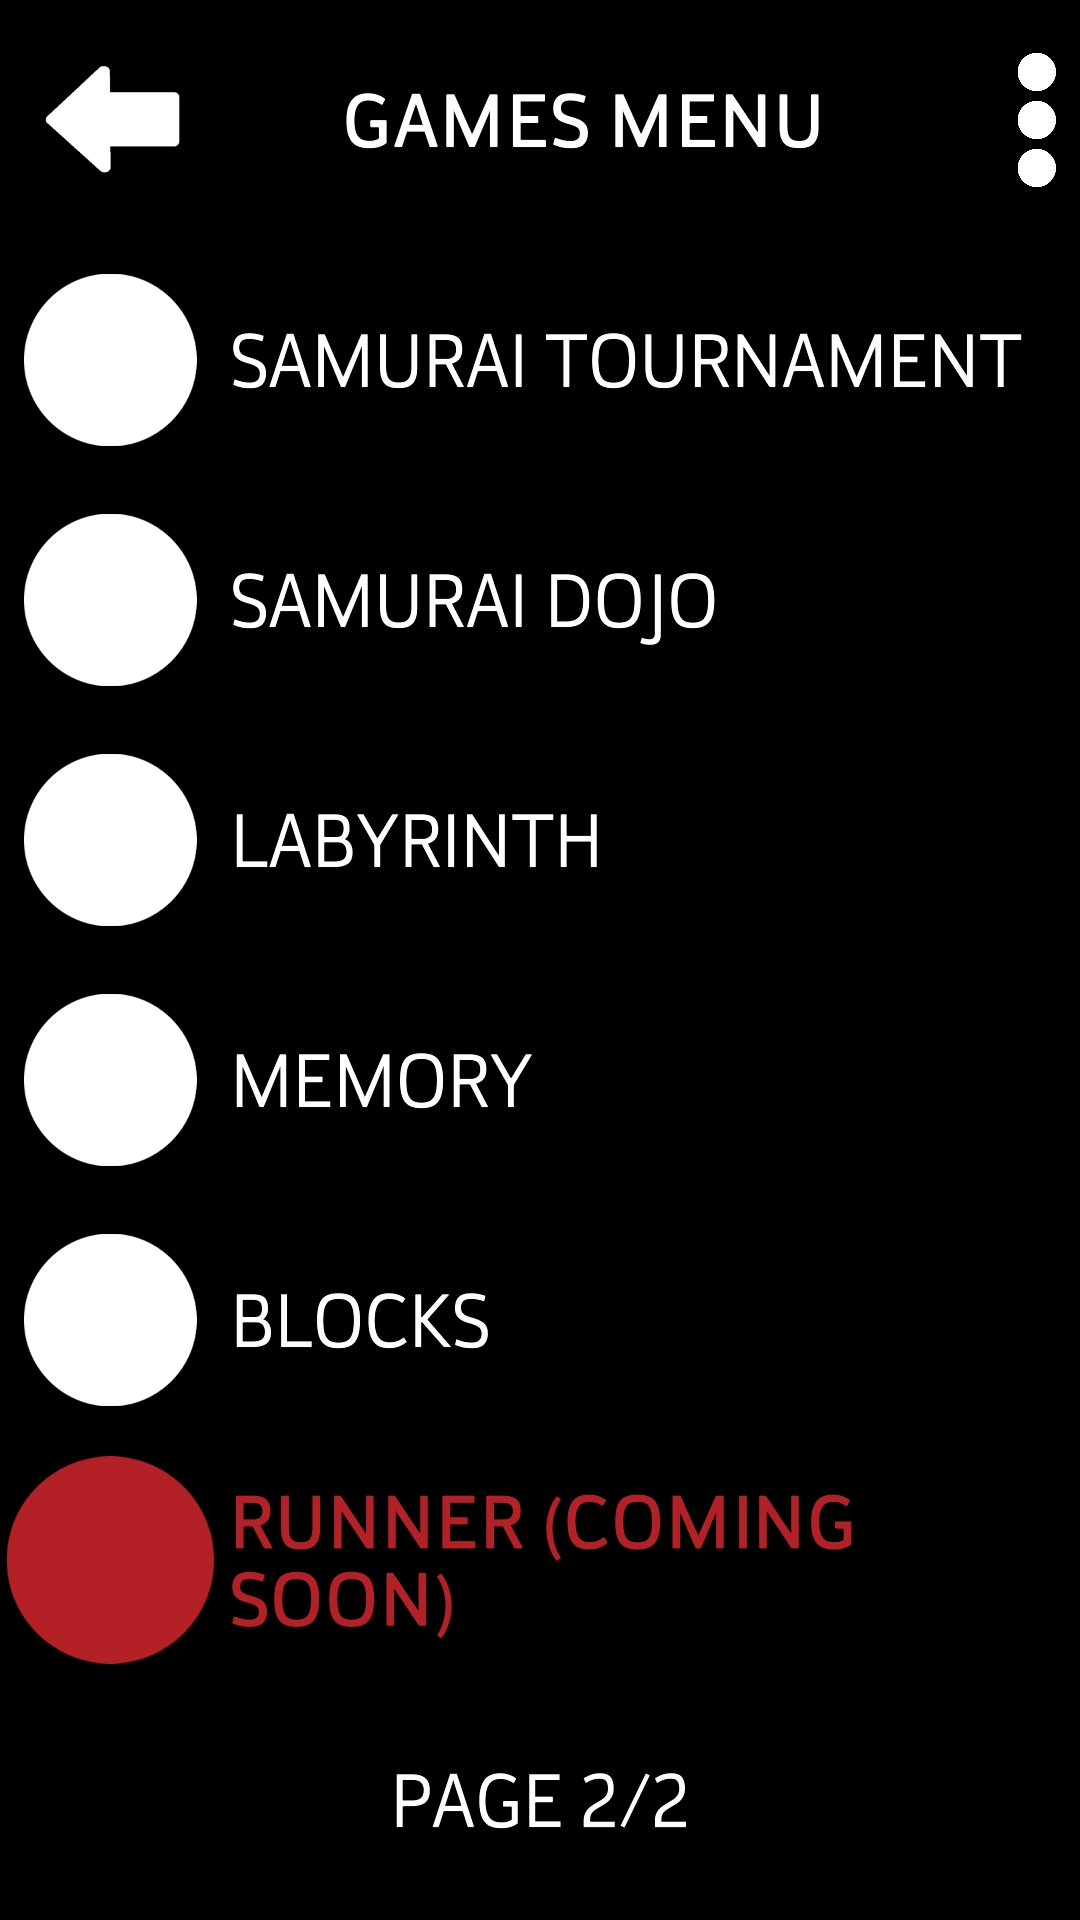
\includegraphics[width=.8\linewidth]{audio hub menu.jpg}
  \caption{audio hub menu}
  \label{fig:audio hub menu}
\end{minipage}%
\begin{minipage}{.5\textwidth}
  \centering
  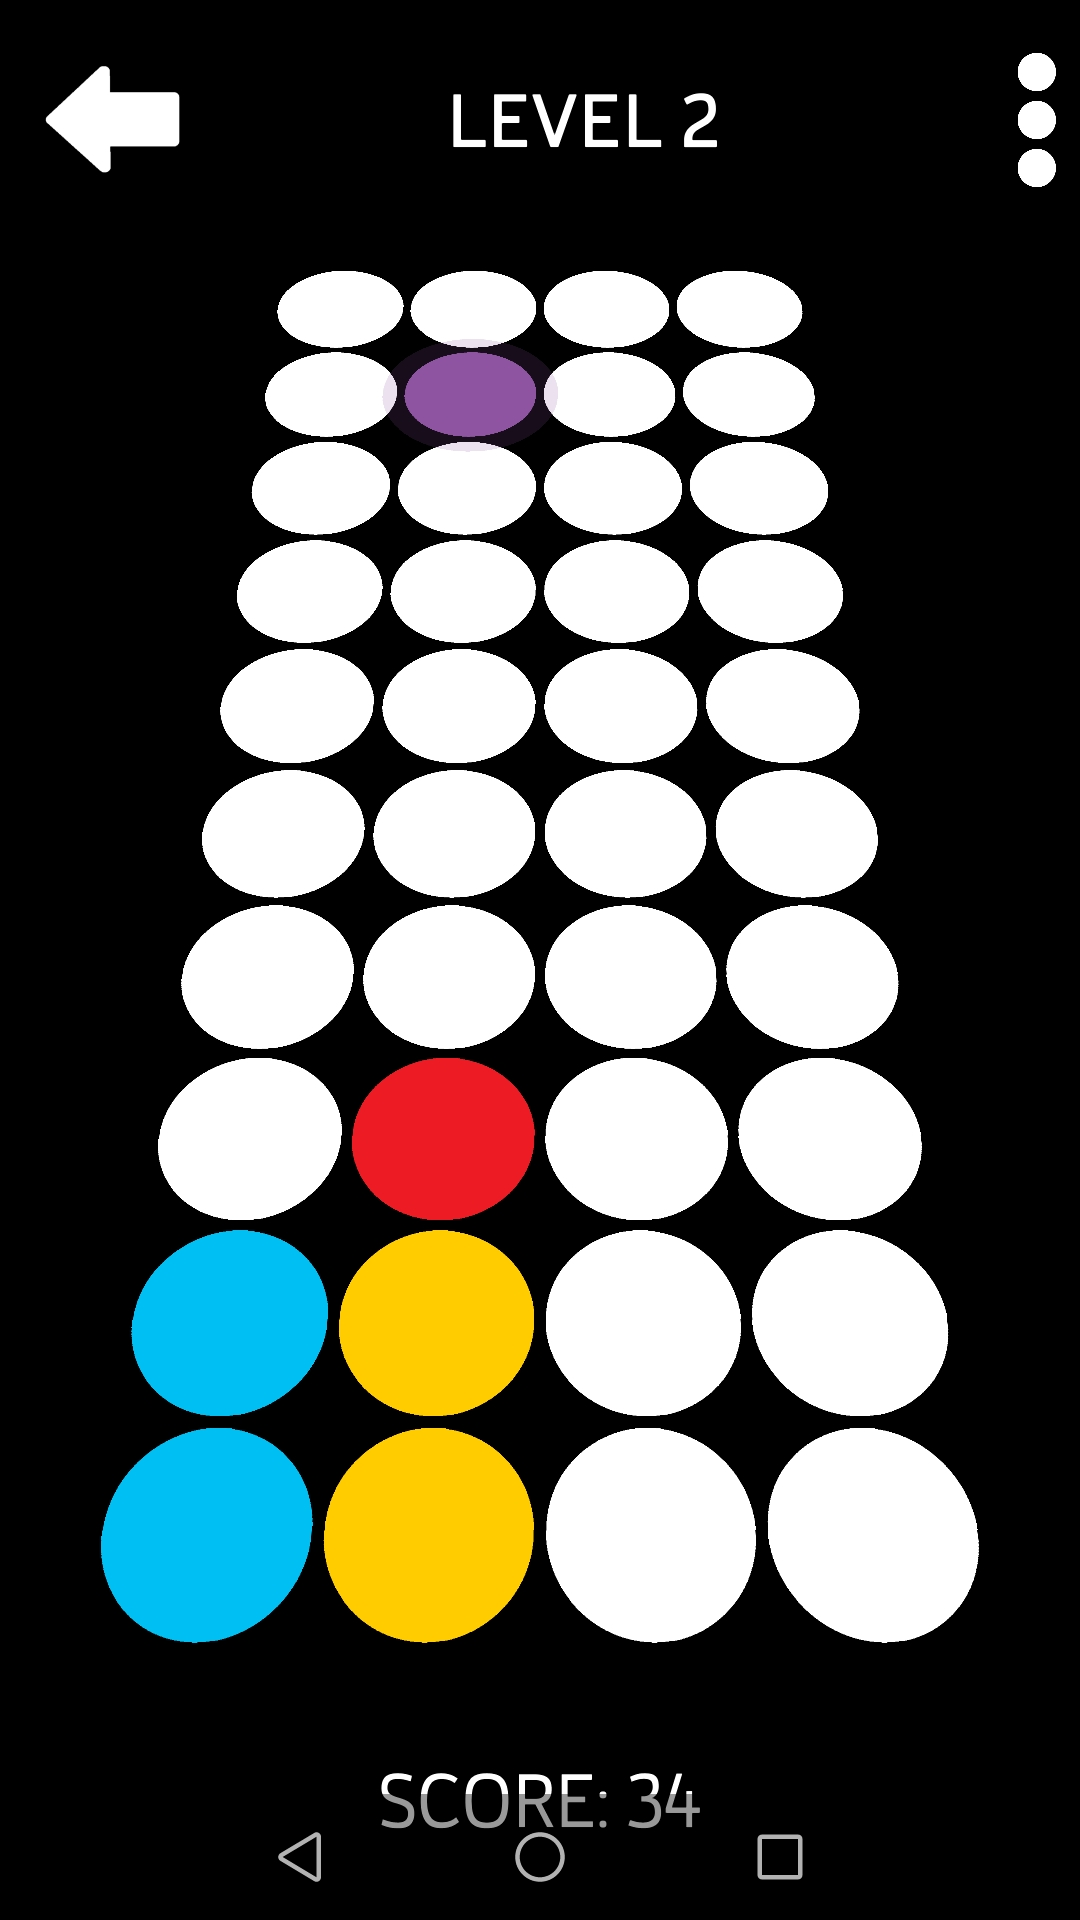
\includegraphics[width=.8\linewidth]{audio hub blocks.jpg}
  \caption{audio hub blocks}
  \label{fig:audio hub blocks}
\end{minipage}
\end{figure}


\chapter{Requirements and tools}

\iffalse
\begin{itemize}
\item functional and nonfunctional requirements
\item use cases (UML diagrams)
\item description of tools
\item methodology of design and implementation
\end{itemize} 

\clearpage
\fi

\section{Functional requirements}
\par
There have been chosen to use both of previously mentioned approaches in the game, by creating a tutorial level with Sudoku 6 by 6 instead of 9 by 9. This way number of elements is decreased by over 55\%, so there are supposed to be two algorithms implemented: one for 6 on 6 and one for 9 on 9. Beside that the application will also need a validation to see if the Sudoku was solved correctly. The use case diagram is shown in \ref{fig:Use case}

\begin{figure}[!hb]
  \centering
  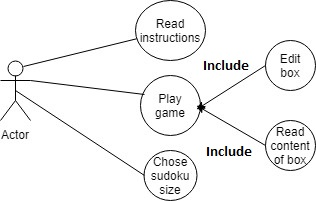
\includegraphics[width=.6\linewidth]{usecase2.jpg}
  \caption{Use case}
  \label{fig:Use case}
\end{figure}

\par
Usage scenario:
%\par
\begin{enumerate}
	\item Instruction on how to play is played to the user(he can skip it if he wants to).
	\item User chose size of the Sudoku.
	\item User fills in the Sudoku.
	\item The program validates if the Sudoku is correct.
\end{enumerate}

\section{Non-functional requirements}
\par
The user interface of the application should work similar to the way that TalkBack is working: 
\begin{itemize}
\item taping an element of Sudoku (number) should result in the interface reading the label to the user;
\item to edit an element, user must hold finger on it for a longer period of time, then the content of the element will be changed to the number that the element was tapped;
\item in both cases, when the user try to edit a starting element (element that the game have started with), or when the user taps an empty element, a short message will be played to inform about it.
\end{itemize}
\par
To make it easier for blind user to find number on the screen of smartphone, and be aware of its localization,
\begin{itemize}
\item it should be possible to zoom in to one cell with only 6 or 9 elements (depending on the type of Sudoku);
\item it would be possible to move between cells by swipe events, and another after zooming out the swipe event can be used to go back to the menu.
\end{itemize}
\par
Other requirements:
\begin{itemize}
\item turning on the TalkBack should not interfere with usage of the application;
\item taking into account that this application can be used also by partially blind people, there can be made a facilitation for them, by displaying white numbers on black background. With this contrast they will be easier to see.
\end{itemize}

\section {Description of tools}%Methodology of design and implementation}

\par The chosen design tool is Android Studio with Java as the chosen programming language. Android Studio have been chosen as the most advanced tool in the field of creating android applications at that time. It is also equipped and compatible with many other useful tools, like emulators that can be used for testing, or plugins generating diagrams. Java was chosen due to the popularity of this programming language, which ensures wither range of existing solutions of many problems.

\par The TTS (Text to speech engine) refers to the ability of device to read text aloud. A TTS Engine converts written text to a phonemic representation, then converts the phonemic representation to wave forms that can be output as sound. TTS engines can be used with different languages, dialects and specialized vocabularies through third-party publishers. Android is fully capable of using them\cite{bib:TTS}.
\par To use TTS in android application all that is necessary is some instance of \lstinline|TextToSpeech|  and use \lstinline|textToSpeech.speak(<string to speak>, TextToSpeech.QUEUE_FLUSH, null);|.

\par Java is a general-purpose computer-programming language that is concurrent, class-based, object-oriented, and specifically designed to have as few implementation dependencies as possible\cite{bib:Java2}. According to Tiobe, Java has been the number 1 or 2 most popular language basically since its creation in the mid-90’s. The popularity of Java helps to ensure its future popularity, thanks to a huge community of users\cite{bib:Java}.

\chapter{External specification}

\iffalse
\begin{itemize}
\item hardware and software requirements
\item installation procedure
%\item activation procedure
\item types of users
\item user manual
%\item system administration
%\item security issues
\item example of usage
\item working scenarios (with screenshots or output files)
\end{itemize}

\clearpage
\fi

\section{Hardware and software requirements}

\par The application requires a device with API 15 or higher version of  Android OS.
Because the whole program uses only basic android functionalitis, there is no point in setting any higher version, this way the application will be available on more devices\cite{bib:book}.


%\section {Installation procedure}

\par
The installation is based on installing the APK file to the device and running the installation procedure appropriate to this device (agreeing on installing applications from unknown source could be needed).

%\section {Activation procedure}

\section{Types of users}
\par This application have been designed having in mind three groups of users:
\begin{itemize}
\item users with no visual disabilities.
\item partially blind users.
\item completely blind users.
\end{itemize}

\par This application has only one universal mode for all types of users. The Sudoku will still have simple visual elements, so the game could be played relying only on the eyesight. The content is read to the user that lets play the game without looking at the screen. And the white on black background contrast could help the partially blind players. This way the application is made as much accessible as it is possible.

\section{User manual}

\par 
All the basic instructions are shown and played every time after starting the application, and can be skipped with tapping the screen. 
\par
Editing the content of Sudoku number is enabled by a long tap, after long tapping the number it can be incremented by tapping it, after reaching the limit the number goes back to zero. Moving between cells to access more numbers is done by swipping a finger on the screen.
\par
When the TalkBack is on, the swipe must be done with two fingers and the long tap have to be preceded with one normal tap as a double tap. All the other functions of the game are the same as with TalkBack off.
\par 
At the beginning user is given a simple instruction on how to play the game:
\begin{quote}
\textit{
Welcome to blind Sudoku!\\*
Fill in the boxes so every number will be placed only
once in every row, column, and cell. Swipe your fingers to navigate between the cells,
and tap a box to hear its content. Long tap the box to enable editing the number, and tap
the box to increment the number. Double tap to continue. Have fun!
}
\end{quote}
\par The way the user interface works was intended to be as similar as possible to the way TalkBack works. So user used to the TalkBack behavior would not have many problems with using it.

%\section{System administration}

%\section {Security issues}

%\section {Example of usage}

\section {Working scenarios with screenshots or output files}

\par This application uses two views:
\begin{itemize}
\item  Instructions (Figure \ref{fig:Game instructions}) - short explanation on how to play the game and use the app. It shows up when the application starts, and can be skipped to go to the game.
\item  Game view (Figure \ref{fig:Sudoku cell}) - the cell filled with numbers from sudoku where zeros are the empty places to be filled in. It starts in the left upper cell of the whole Sudoku matrix.
\end{itemize}

\iffalse
\begin{figure}
\centering
  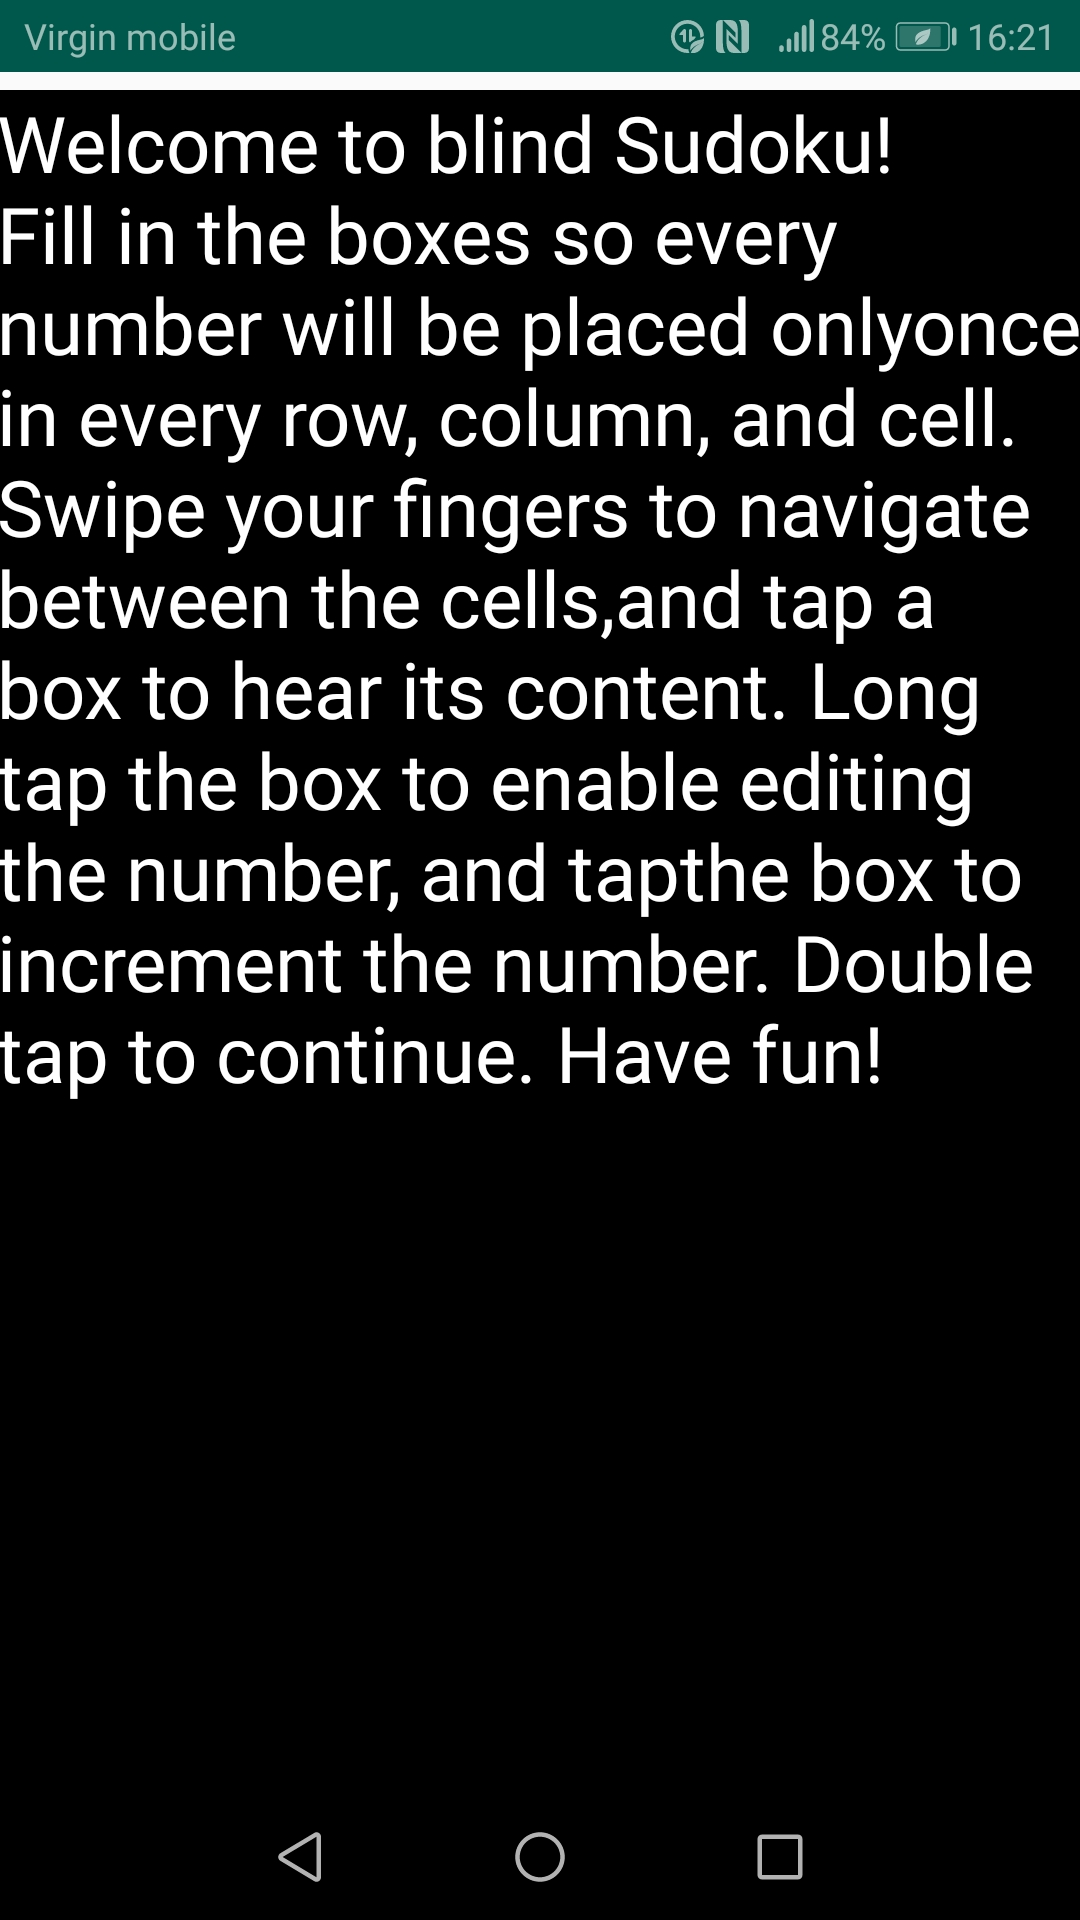
\includegraphics[width=\linewidth/2]{instructions.jpg}
  \caption{Instructions.}
  \label{fig:Game instructions}
%\end{centering}
\end{figure}

Figure \ref{fig:Game instructions} shows a welcome message with instructions how to use the application and solve the sudoku.

\begin{figure}[H]
\centering
  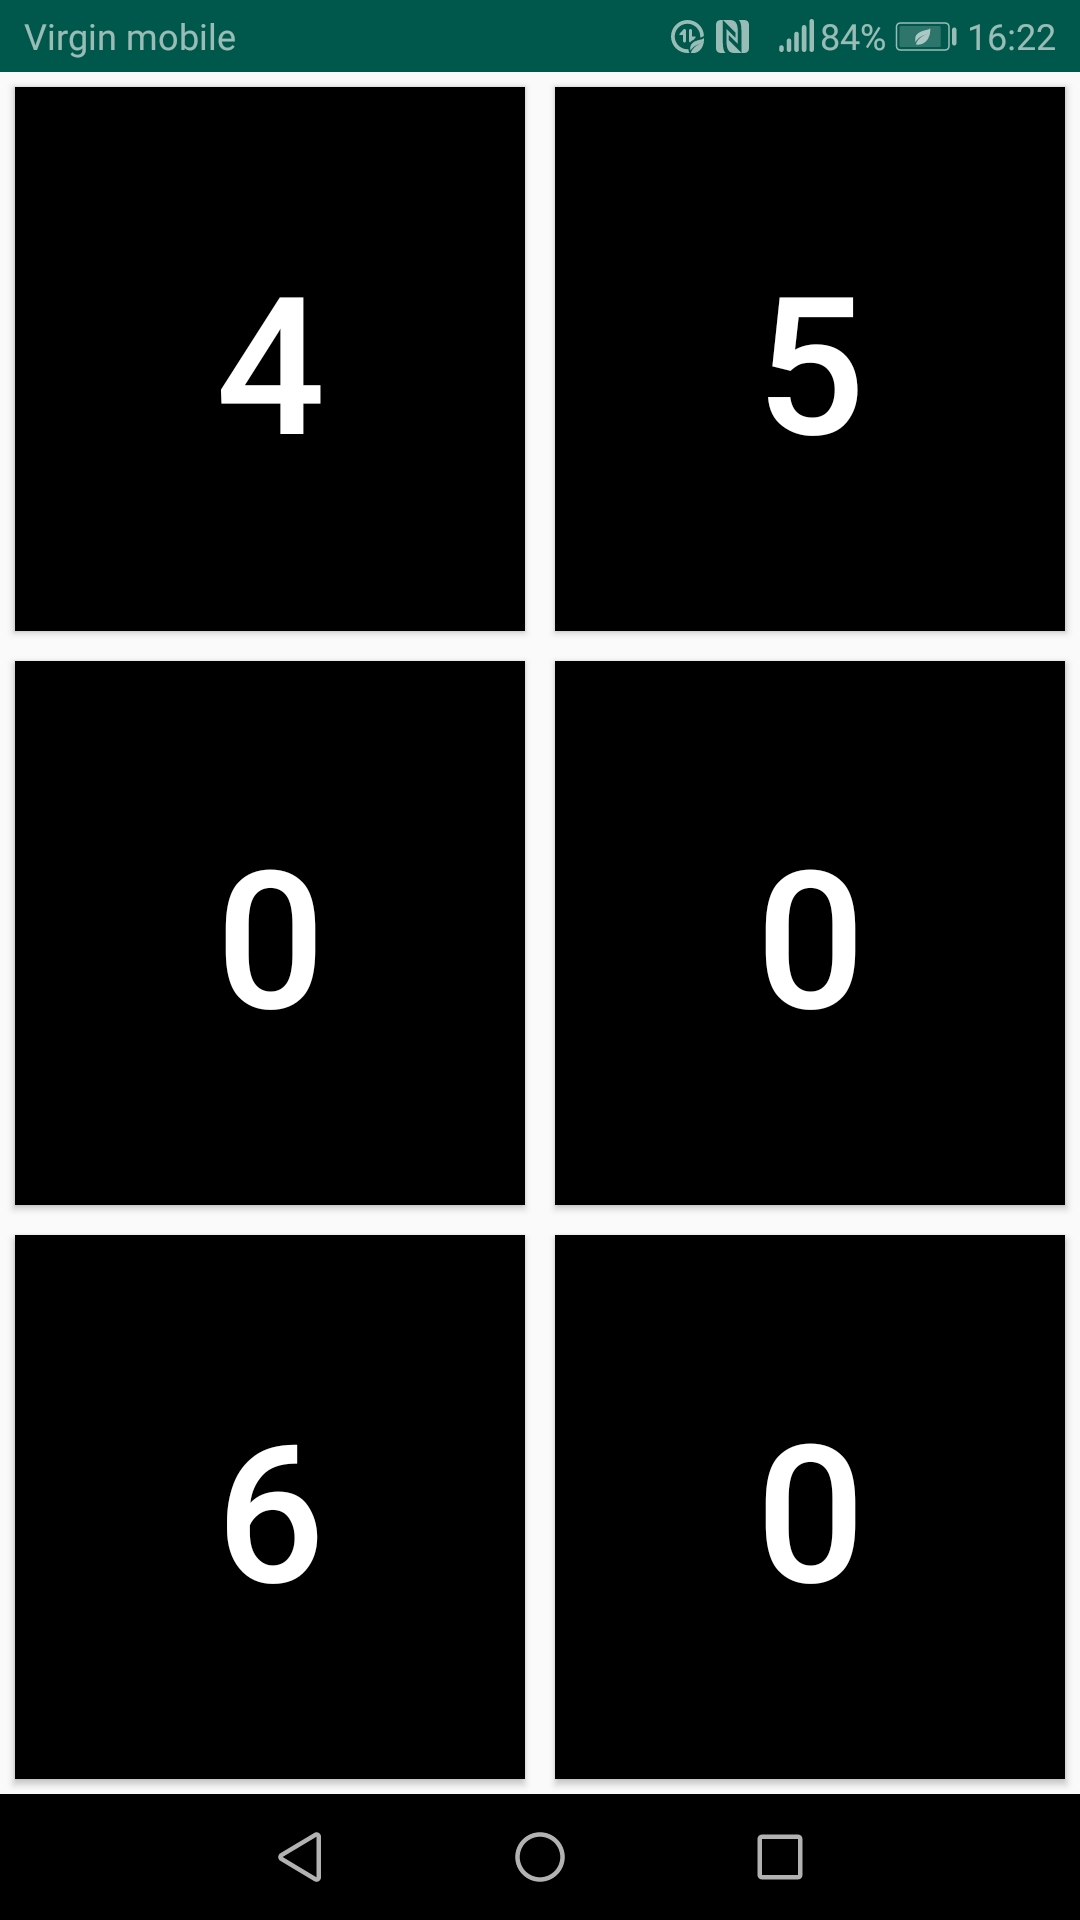
\includegraphics[width=\linewidth/2]{sudoku cell.jpg}
  \caption{Sudoku cell.}
  \label{fig:Sudoku cell}
%\end{centering}
\end{figure}

Figure \ref{fig:Sudoku cell} shows a Sudoku cell with six number boxes, where zeros are the empty boxes. 
\fi

\begin{figure}[H]
\centering
\begin{minipage}{.5\textwidth}
  \centering
  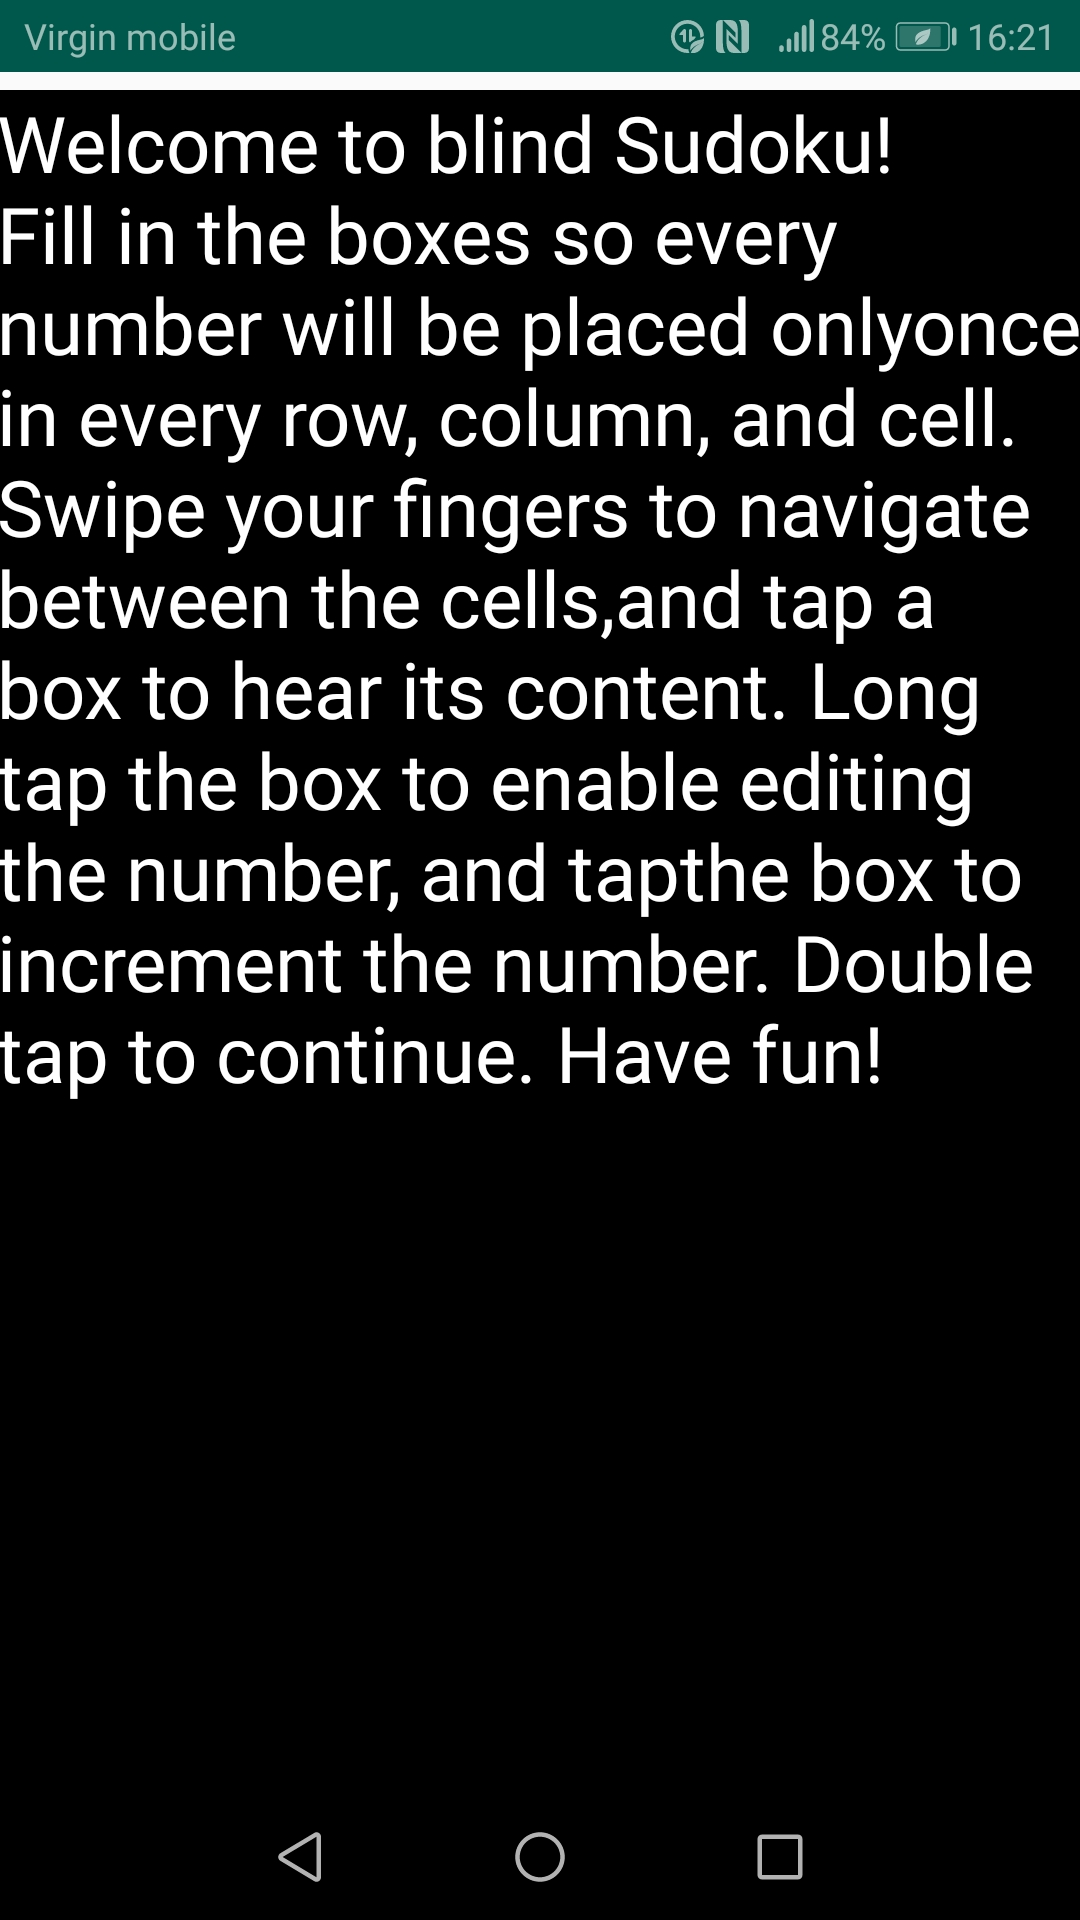
\includegraphics[width=.8\linewidth]{instructions.jpg}
  \caption{Instructions}
  \label{fig:Game instructions}
\end{minipage}%
\begin{minipage}{.5\textwidth}
  \centering
  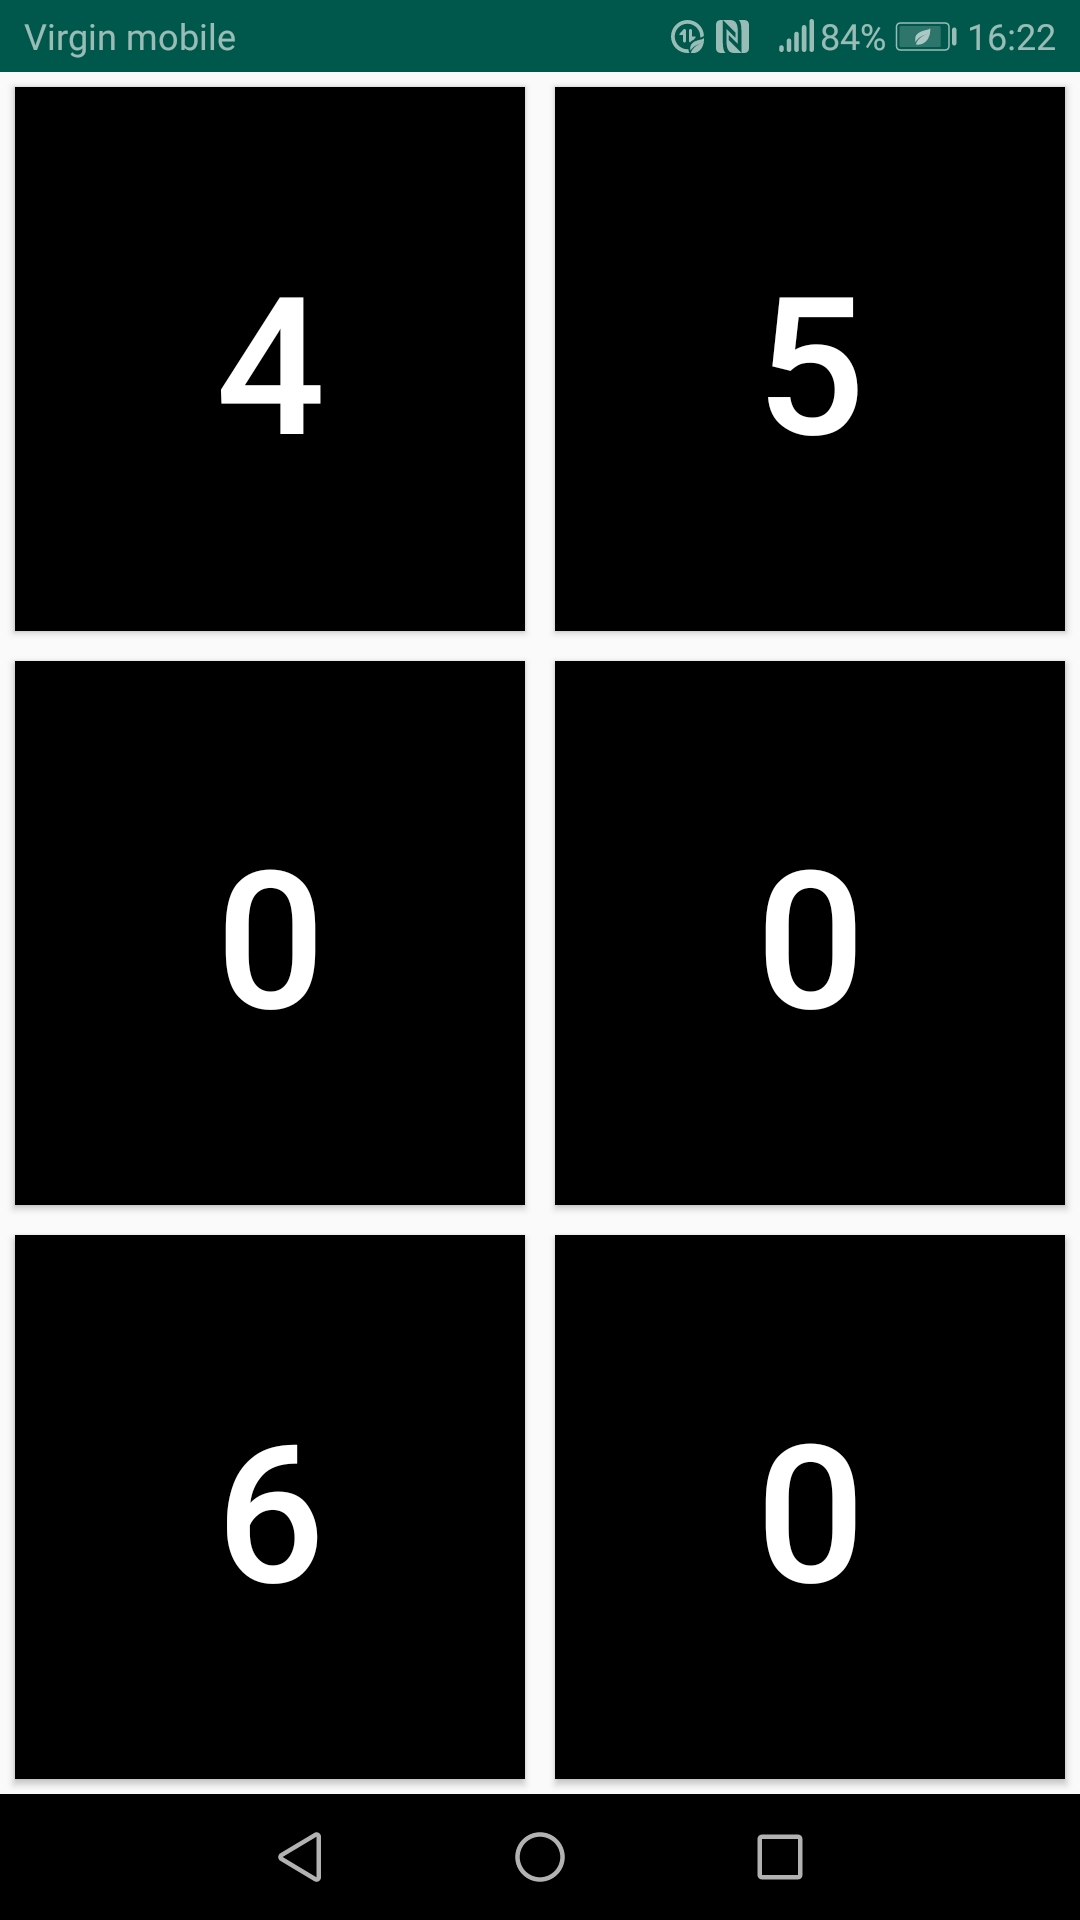
\includegraphics[width=.8\linewidth]{sudoku cell.jpg}
  \caption{Sudoku cell}
  \label{fig:Sudoku cell}
\end{minipage}
\end{figure}



\chapter{Internal specification}

\iffalse
\begin{itemize}
%\item concept of the system
%\item system architecture
%\item description of data structures (and data bases)
\item components, modules, libraries, resume of important classes (if used)
\item resume of important algorithms (if used)
\item details of implementation of selected parts
\item applied design patterns
\item UML diagrams
\end{itemize}


Use special environment for inline code, eg \lstinline|descriptor| or \lstinline|descriptor_gaussian|. 
Longer parts of code put in the figure environment, eg. code in Fig. \ref{fig:pseudokod}. Very long listings–move to an appendix.

\clearpage
\fi

%\section {Concept of the system}
%\section {System architecture}
%\section {Description of data structures }
\section {Class architecture}

\par
The whole program is based mostly on two classes. The sudoku data processing in class Sudoku made of: generating Sudoku, validating the Sudoku, and all the other methods needed to work with the Sudoku. The \lstinline|MainActivity| class responsible for using the Sudoku class and connecting it to the other elements of the game.
\par Instead of creating additional activity for the view with instructions (that only would handle one action), application uses only the \lstinline|MainActivity| changing the XML file it uses as the current view.

\begin{figure}[H]
\centering
  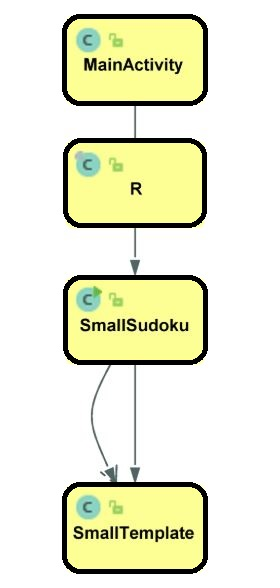
\includegraphics[width=\linewidth/2]{UML.jpg}
  \caption{UML diagram.}
  \label{fig:Diagram}
%\end{centering}
\end{figure}

Figure \ref{fig:Diagram} UML of the project.

\par The application is based mostly on 3 classes:
\begin{itemize}

\item \lstinline|MainActivity| - the activity of this application.
\item \lstinline|SmallSudoku| - matrix with Sudoku data, and useful methods.
\item \lstinline|SmallTemplate| - template used to determine which numbers are removed from the Sudoku matrix at the beginning of game.

\end{itemize}

\section {Resume of important algorithms}
\par
Generation of the 6 by 6 Sudoku was problematic, due to the fact that a square cannot be made of six square elements (what is required by most algorithms). This is why this program uses a simpler algorithm:
\begin{enumerate}
	\item Generate numbers from one to six in random order, and put them into the first row.
	\item Go to the next row.
	\item Copy the content of the previous row and: 
	\begin{enumerate}
   		 \item If the row number can be divided by 3, shift the numbers of this row by one place.
   		 \item If the row number can not be divided by 3, shift the numbers of this row by two places.
  	\end{enumerate}
	\item If the Sudoku is not full yet, go back to step number two.
	\item The Sudoku is ready.
\end{enumerate}

\par Later on the generated data is copied from one array to another during the copping process the correct indexes of the arrays are compared with a ready made \lstinline|SmallTemplate| object to create holes for the user to fill in. Letters on both the first and the second array can be compared to see it the user solved the second correctly.



\section {Details of implementation of selected parts}

\par The game is based mostly on only one view in form of XML file, that is one Sudoku cell, with numbers changing after moving between cells, and editing the content inside them. After every swipe the current cell number is adjusted and the function updating the view, with data from Sudoku, is called.
\par The application behavior with TalkBack should be similar to the one with TalkBack turned off as much as possible. Firstly the reading of buttons labels by TalkBack was turned off, so it would be done by the implementation in the program. It was done by setting buttons \lstinline|android:importantForAccessibility| to "no" in the XML file, as seen on figure \ref{fig:Button}.


\begin{figure}[H]
\centering
\begin{lstlisting}
<Button
            android:importantForAccessibility="no"
            android:id="@+id/button"
            android:tag="0"
            android:layout_width="0dip"
            android:layout_height="match_parent"
            android:background="#000000"
            android:text="0"
            android:textSize="64dp"
            android:textColor="#FFFFFF"
            android:layout_margin="5dp"
            android:layout_weight="1" />
\end{lstlisting}
\caption{The \lstinline|button| element from MainActivity.xml}
\label{fig:Button}
\end{figure}


\par Secondly the reaction to tapping the buttons had to be overeaten, so the user would not have to tap twice more times and to override the previously mentioned reading of labels. It was done by using the setOnHoverListener on buttons, and implementing there the same behavior as in the onClick method, where we test if the TalkBack is on by using the AccessibilityManager.


%\section {Applied design patterns}
%\section {UML diagrams}




\chapter{Verification and validation}

\iffalse
\begin{itemize}
\item testing paradigm (eg V model)
\item test cases, testing scope (full / partial)
\item detected and fixed bugs
\item results of experiments (optional)
\end{itemize}

 \clearpage
\fi

\section{Testing paradigm}

\par Due to the fact that the most crucial features could not been tested by means of unit testing nor integration testing (behavior with TalkBack, audio messages), the only performed testing was acceptance testing.
\par According to the V-model (as shown on figure \ref{fig:model}\cite{inproceedings}) the testing should include unit testing, integration testing, system testing, and user acceptance testing. But (as written above) due to internal architecture of the application it was possible to perform the last type of testing.

\begin{figure}[H]
\centering
  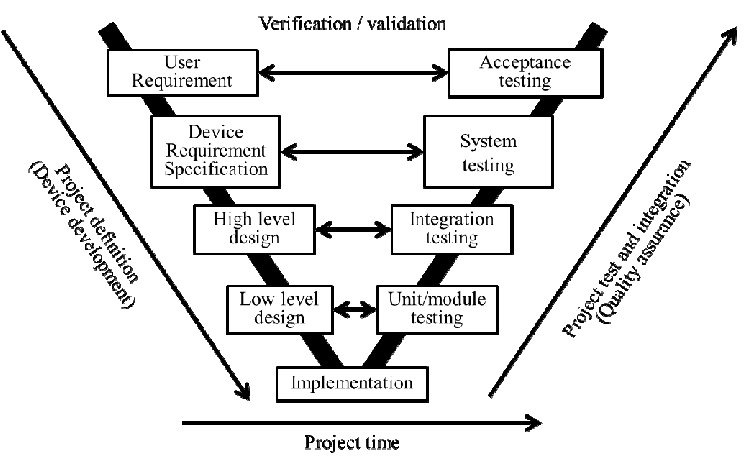
\includegraphics[width=.8\linewidth]{V-model.png}
  \caption{V-model.}
  \label{fig:model}
%\end{centering}
\end{figure}

\par After implementing each functionality it was tested manually on a smartphone.

\section{Test cases}

\par During the manual testing there were taken into account some crucial features and their behavior. They are described in the table \ref{usecase:Table} cases in testing.

\iffalse
\begin{table}[H]
\label{table:Table}
\begin{tabular}
%\hline
\rowcolor{lightgray}\multicolumn{2}{|c|}{Use cases} \\
\hline
Action & Result\\
\hline
Edit empty box & After long tapping the empty box the number editing is enabled, and every tap increments the number. After next long tap the content of box is saved.\\
\hline
Edit box with content generated by application & User is informed that the content cannot be changed.\\
\hline
Single tap a box & Application speaks the number that is inside the box.\\
\hline
Single tap a box when TalkBack is on & Application speaks the number that is inside the box.\\
\hline
Swipe vertically and horisontally & The view moves between cells and stops and detects if it can move further.\\
\hline
Fill in the Sudoku correctly & Application informs that the Sudoku is correct.\\
\hline
Fill in the Sudoku incorrectly & Application informs that the Sudoku is incorrect.
\end{tabular}
\end{table}
\fi

%\iffalse
\begin{usecase}{User actions}{Result}
	\label{usecase:Table}
    \addrow{Edit empty box}{After long tapping the empty box the number editing is enabled, and every tap increments the number. After next long tap the content of box is saved.}

    \addrow{Edit box with content generated by application}{User is informed that the content cannot be changed.}

	\iffalse
    \addmulrow{Main path (M)}{
        \item User selects \ldots
        \item System demands \ldots}
	\fi
	\addrow{Single tap a box}{Application speaks the number that is inside the box.}
	\addrow{Single tap a box when TalkBack is on}{Application speaks the number that is inside the box.}
	\addrow{Swipe vertically and horisontally}{The view moves between cells and stops and detects if it can move further.}
	\addrow{Fill in the Sudoku correctly}{Application informs that the Sudoku is correct.}
	\addrow{Fill in the Sudoku incorrectly}{Application informs that the Sudoku is incorrect.}
	
\end{usecase}
%\fi

\section{Detected and fixed bugs}

\par During the development and the actual testing procedure, there have been found and fixed fallowing bugs:
\begin{itemize}
	\item The upper limit for vertival cell movement was to high, that resulted in index out of bounds exception.
	\item The application was displaying wrong numbers due to a mistake in translation of button number into x and y coordinates of sudoku.
	\item Vertical swipe was not always working, because the event was not defined properly.
	\item Application was not able to compile. The first usage of the text to speech was accidentally before its initialization.
\end{itemize}

\par Due to the importance of TalkBack compatibility, every feature had to be tested with and without enabled TalkBack.

\chapter{Conclusions}

\iffalse
\begin{itemize}
\item achieved results with regard to objectives of the thesis and requirements
\item path of further development (eg functional extension …)
\item encountered difficulties and problems
\end{itemize}
\fi

%\clearpage

\section{Achieved results}% with regard to objectives of the thesis and requirements}

%changed
\iffalse
\par The most important objectives of this thesis were:
\begin{itemize}
\item Having Sudoku puzzle that is possible to solve for a user with a visual disability.
\item The visual elements should be letting a partially blind user and fully sighted user to solve the puzzle using them.
\item Behavior of application with TalkBack turned on, and with the TalkBack turned off should not differ in many details.
\end{itemize}
\fi

\par In the chapter one section Objective of the thesis, and chapter three Functional requirements and Non-functional requirements have been stated objectives and expectations towards the thesis. Here is description of meet requirements.
\begin{itemize}

\item In this mobile game there is generated sudoku puzzle.
\item User can chose between 6 on 6 and 9 on 9 sizes of sudoku.
\item Colors are in contrast helping partially blind users.
\item  Sudoku can be solved without looking at the screen.
\item Editing box with content generated by application is blocked, but editing empty box is possible.
\item Single tapping a box results in application speaking the number that is inside the box .
\item Application works mostly the same with TalkBack on and TalkBack off.
\item Only one cell is shown at a time and moving between cells is done by swipping the screen.
\item After filling in the whole Sudoku applications checks if it is correct.

\end{itemize}



\iffalse
\begin{usecase}{Is it expected result}[bp!]
\label{usecase:result}
%\addrow{Expected result}{Final result}
\addrow{There is generated sudoku puzzle}{Yes.}
\addrow{Editing box with content generated by application is blocked, but editing empty box is possible}{Yes.}
\addrow{Single tapping a box results in application speaking the number that is inside the box }{Yes.}
\addrow{Application works the same with TalkBack on and TalkBack off}{When the TalkBack is off editing box is enabled by long tapping the box, and with TalkBack on it is enabled by double long tapping the box.}
\addrow{Only one cell is shown at a time and moving between cells is done by swipping the screen.}{Yes.}
\addrow{After filling in the whole Sudoku applications checks if it is correct.}{Yes.}
\addrow{Sudoku can be solved without looking at the screen}{Yes.}
\addrow{User can chose between 6 on 6 and 9 on 9 sizes of sudoku}{No.}
\addrow{Colors are in contrast helping partially blind users.}{Yes.}
\addrow{The main objectives of the thesis are meet.}
\end{usecase}
\fi


\par The final result of the project is fully functional Sudoku mobile game that can be played without looking at the screen. It can work both with and without the TalkBack turned on, and the accessibility feature would not change. The only difference in playing the game with TalkBack turned on is the way player enables the change of number in button. Instead of just holding the button for a longer period of time, it must be double tapped where the second tap is the one to be held longer.

\section{Path of further development}

\par At this time the game can be played only on small (six on six) Sudoku with simple algorithm of generation, for better game play results it could be possible to chose size of Sudoku and difficulty level. The application could be also extended by additional features not necessary for the game mechanics like saving time of the play into a ranking to compere results. Possibility to see the ranking should be made in the menu view, that would be also useful to implement together with going back to menu from the game view.
\par There are also other features that could make the game more accessible. Possibility of showing the whole Sudoku on the screen, by making the zoom out gesture, and zoom in to go back into the single cell. When the whole Sudoku is visible it is easier to look thru rows and columns, but navigating between 36 elements (or even 81 if the nine on nine version was chosen) could be challenging for a blind person, so both zoom in and zoom out views should be available. Similar result can be achieved by implementing hints for the user: Telling him if there is a certain number in a row or column. How many occurrences of a certain numbers missing in the whole Sudoku. It could also read all numbers in a row or column in the same order as they are placed in the Sudoku.
\par Leaving the subject of the game itself, there is also place for improvement in the displaying the text. The contrast of white text on black background can help people who still have partial sight, but for large variety of eyesight diseases, it can be possible that for some eyesight disease it would be easier to read with different contrast. This is why it should be possible to change the colors of contrast in the menu settings.

\section{Encountered difficulties and problems}

\par The most difficult part of implementing this application was making the application behavior, with and without TalkBack, as similar as possible. There were many aspects that had to be taken into account, as many normal behaviors of the phone are overwritten when the TalkBack is on.
\par The second most difficult part of implementing this application was coming up with easy and intuitive user interface, that would not include many inconveniences for visually disabled users.

 \iffalse
\begin{table}
\centering
\caption{A caption of a table is \textbf{above} it.}
\label{id:tab:wyniki}
\begin{tabular}{rrrrrrrr}
\toprule
	         &                                     \multicolumn{7}{c}{method}                                      \\
	         \cmidrule{2-8}
	         &         &         &        \multicolumn{3}{c}{alg. 3}        & \multicolumn{2}{c}{alg. 4, $\gamma = 2$} \\
	         \cmidrule(r){4-6}\cmidrule(r){7-8}
	$\zeta$ &     alg. 1 &   alg. 2 & $\alpha= 1.5$ & $\alpha= 2$ & $\alpha= 3$ &   $\beta = 0.1$  &   $\beta = -0.1$ \\
\midrule
	       0 &  8.3250 & 1.45305 &       7.5791 &    14.8517 &    20.0028 & 1.16396 &                       1.1365 \\
	       5 &  0.6111 & 2.27126 &       6.9952 &    13.8560 &    18.6064 & 1.18659 &                       1.1630 \\
	      10 & 11.6126 & 2.69218 &       6.2520 &    12.5202 &    16.8278 & 1.23180 &                       1.2045 \\
	      15 &  0.5665 & 2.95046 &       5.7753 &    11.4588 &    15.4837 & 1.25131 &                       1.2614 \\
	      20 & 15.8728 & 3.07225 &       5.3071 &    10.3935 &    13.8738 & 1.25307 &                       1.2217 \\
	      25 &  0.9791 & 3.19034 &       5.4575 &     9.9533 &    13.0721 & 1.27104 &                       1.2640 \\
	      30 &  2.0228 & 3.27474 &       5.7461 &     9.7164 &    12.2637 & 1.33404 &                       1.3209 \\
	      35 & 13.4210 & 3.36086 &       6.6735 &    10.0442 &    12.0270 & 1.35385 &                       1.3059 \\
	      40 & 13.2226 & 3.36420 &       7.7248 &    10.4495 &    12.0379 & 1.34919 &                       1.2768 \\
	      45 & 12.8445 & 3.47436 &       8.5539 &    10.8552 &    12.2773 & 1.42303 &                       1.4362 \\
	      50 & 12.9245 & 3.58228 &       9.2702 &    11.2183 &    12.3990 & 1.40922 &                       1.3724 \\
\bottomrule
\end{tabular}
\end{table}  
\fi
 

 


%%%%%%%%%%%%%%%%%%%%%%%%%%%%%%%%%%%%%%%%%%
\backmatter
\pagenumbering{Roman}
\stepcounter{PagesWithoutNumbers}
\setcounter{page}{\value{PagesWithoutNumbers}}

\pagestyle{onlyPageNumbers}

%%%%%%%%%%% bibliography %%%%%%%%%%%%
\bibliographystyle{plain}
\bibliography{bibliography}

%%%%%%%%%  appendices %%%%%%%%%%%%%%%%%%% 

\begin{appendices} 


 

\chapter*{List of abbreviations and symbols}

\begin{itemize}
\item[DNA] deoxyribonucleic acid
\item[MVC] model--view--controller 
\item[$N$] cardinality of data set
\item[$\mu$] membership function of a fuzzy set
\item[$\mathbb{E}$] set of edges of a graph
\item[$\mathcal{L}$] Laplace transformation
\end{itemize}


\chapter*{Listings}

(Put long listings in the appendix.)


\iffalse
\begin{lstlisting}
partition fcm_possibilistic::doPartition
                             (const dataset & ds)
{
   try
   {
      if (_nClusters < 1)
         throw std::string ("unknown number of clusters");
      if (_nIterations < 1 and _epsilon < 0)
         throw std::string ("You should set a maximal number of iteration or minimal difference -- epsilon.");
      if (_nIterations > 0 and _epsilon > 0)
         throw std::string ("Both number of iterations and minimal epsilon set -- you should set either number of iterations or minimal epsilon.");
   
      auto mX = ds.getMatrix();
      std::size_t nAttr = ds.getNumberOfAttributes();
      std::size_t nX    = ds.getNumberOfData();
      std::vector<std::vector<double>> mV;
      mU = std::vector<std::vector<double>> (_nClusters);
      for (auto & u : mU)
         u = std::vector<double> (nX);
      randomise(mU);
      normaliseByColumns(mU);
      calculateEtas(_nClusters, nX, ds);
      if (_nIterations > 0)
      {
         for (int iter = 0; iter < _nIterations; iter++)
         {
            mV = calculateClusterCentres(mU, mX);
            mU = modifyPartitionMatrix (mV, mX);
         }
      }
      else if (_epsilon > 0)
      {
         double frob;
         do 
         {
            mV = calculateClusterCentres(mU, mX);
            auto mUnew = modifyPartitionMatrix (mV, mX);
            
            frob = Frobenius_norm_of_difference (mU, mUnew);
            mU = mUnew;
         } while (frob > _epsilon);
      }
      mV = calculateClusterCentres(mU, mX);
      std::vector<std::vector<double>> mS = calculateClusterFuzzification(mU, mV, mX);
      
      partition part;
      for (int c = 0; c < _nClusters; c++)
      {
         cluster cl; 
         for (std::size_t a = 0; a < nAttr; a++)
         {
            descriptor_gaussian d (mV[c][a], mS[c][a]);
            cl.addDescriptor(d);
         }
         part.addCluster(cl);
      }
      return part;
   }
   catch (my_exception & ex)                                  
   {                                                       
      throw my_exception (__FILE__, __FUNCTION__, __LINE__, ex.what()); 
   }                                                          
   catch (std::exception & ex)                                 
   {                                                            
      throw my_exceptionn (__FILE__, __FUNCTION__, __LINE__, ex.what()); 
   }                                                            
   catch (std::string & ex)                                     
   {                                                            
      throw my_exception (__FILE__, __FUNCTION__, __LINE__, ex);        
   }                                                             
   catch (...)                                                   
   {                                                             
      throw my_exception (__FILE__, __FUNCTION__, __LINE__, "unknown expection");       
   }  
}
\end{lstlisting} 
\fi

\chapter*{Contents of attached CD}

The thesis is accompanied by a CD containing:
\begin{itemize}
\item thesis (\LaTeX\ source files and final \texttt{pdf} file),
\item source code of the application,
\item test data.
\end{itemize}
 

\listoffigures
\listoftables
	
\end{appendices}


\end{document}


%% Finis coronat opus.